
%========= File containing the main LaTex document ========%
%                                                          %
% Copyright (C) ISI - All Rights Reserved                  %
% Proprietary                                              %
% Written by Med Hossam <med.hossam@gmail.com>, April 2016 %
%                                                          %
% @author: HEDHILI Med Houssemeddine                       %
% @linkedin: http://tn.linkedin.com/in/medhossam           %
%==========================================================%

%\documentclass[pfe]{./tpl/isipfe}
\documentclass[]{./tpl/isipfe}
\graphicspath{{./img/}}

%\usepackage{hyperref}
\usepackage{graphicx}
\usepackage{float}
\usepackage{amsmath}
\usepackage{amssymb}
\usepackage{booktabs}
\usepackage{longtable}
\usepackage{array}
\usepackage{multirow}
\usepackage{xcolor}
\usepackage{listings}
\usepackage{hyperref}
\usepackage{caption}
\usepackage{subcaption}
\usepackage{tikz}
\usepackage{pgfplots}
\pgfplotsset{compat=1.18}
\usepackage{fancyhdr}
\usepackage{titlesec}
\usepackage{enumitem}
\usepackage{algorithm}
\usepackage{algpseudocode}
\usepackage{cite}
\usepackage{url}
\usepackage{microtype}
\usepackage[space]{grffile}

% ── Color definitions ──────────────────────────────────────────────
\definecolor{codeblue}{RGB}{37,99,235}
\definecolor{codegray}{RGB}{100,116,139}
\definecolor{codebg}{RGB}{248,250,252}
\definecolor{accent}{RGB}{37,99,235}
\definecolor{detcolor}{RGB}{8,145,178}
\definecolor{clscolor}{RGB}{22,163,74}
\definecolor{armcolor}{RGB}{124,58,237}

% ── TikZ libraries ─────────────────────────────────────────────────
\usetikzlibrary{arrows.meta, shapes.geometric, positioning, fit, calc}

% ── Code listing style ─────────────────────────────────────────────
\lstdefinestyle{pythonstyle}{
    backgroundcolor=\color{codebg},
    commentstyle=\color{codegray}\itshape,
    keywordstyle=\color{codeblue}\bfseries,
    numberstyle=\tiny\color{codegray},
    stringstyle=\color{clscolor},
    basicstyle=\ttfamily\footnotesize,
    breakatwhitespace=false,
    breaklines=true,
    captionpos=b,
    keepspaces=true,
    numbers=left,
    numbersep=5pt,
    showspaces=false,
    showstringspaces=false,
    showtabs=false,
    tabsize=2,
    frame=single,
    rulecolor=\color{codegray!40},
}
\lstset{style=pythonstyle}

\input{./tpl/new_commands}

% @author: Stoufa
% the command `\makeindex` is mandatory to create the index file main.idx
% https://tex.stackexchange.com/questions/9913/input-index-file-not-found
\makeindex


\AtBeginDocument{%
  \selectlanguage{english}%
}
% Fix mini table of contents title
\mtcsettitle{minitoc}{Contents}
% Change table/figure caption names
\captionsetup[table]{name=Table}
\captionsetup[figure]{name=Figure}

\makeindex


\begin{document}
\mtcselectlanguage{english}       % Tell minitoc to use English
\selectlanguage{english}          % Tell babel to use English
\renewcommand{\contentsname}{Table of Contents}   % Final safeguard
    
%=== File containing Global Configuration of the report ===%
%                                                          %
% Copyright (C) ISI - All Rights Reserved                  %
% Proprietary                                              %
% Written by Med Hossam <med.hossam@gmail.com>, April 2016 %
%                                                          %
% @author: HEDHILI Med Houssemeddine                       %
% @linkedin: http://tn.linkedin.com/in/medhossam           %
%==========================================================%

%=========== You MUST type your information here ==========%
% global_config.tex file is designed to configure your     %
% cover pages (main, back and black covers)                %
%==========================================================%

%============= Config new columns type ==============%
\newcolumntype{L}{>{\raggedright\arraybackslash}}
\newcolumntype{R}{>{\raggedleft\arraybackslash}}
\newcolumntype{C}{>{\centering\arraybackslash}}
%==================================================%

%========= Config the cover section ==========%

\title{Comparative assessment of hardware accelaration on the Edge AI }

\author{Walid Ben Abi Taieb}
%%% if necessary
% Set isBinomal to true and type second author name
%\setboolean{isBinomal}{true}
%\secondAuthor{Prénom NOM}

\diplomaName{National Diploma of Engineering in Applied Science Technology}
\speciality{Embedded Systems and Connected Objects}
%\speciality{Génie des Télécommunications et Réseaux}
%\speciality{Génie Informatique des Systèmes Industriels}

%% Encadrant professionnel
\proFramerName{Mr. Enrico Mezzetti }
\proFramerSpeciality{}

%% Encadrant académique
\academicFramerName{Mrs. Mariem Feki}
\academicFramerSpeciality{}

%% Entreprise d'accueil
\companyName{Barcelona supercomputing center }

%% Année universitaire
\collegeYear{2025 - 2026}

%%%%%% Signatures section %%%%%%

% You can simply remove theses sentences by typing an empty string
% \proSignSentence{}

\proSignSentence{I authorize the student to submit their internship report for validation.}

\academicSignSentence{I authorize the student to submit their internship report for validation.}

%%% AR
\arabicAbstract{يوضع الملخص باللغة العربية هنا... يوضع الملخص باللغة العربية هنا... يوضع الملخص باللغة العربية هنا... يوضع الملخص باللغة العربية هنا... يوضع الملخص باللغة العربية هنا... الرجاء أن يكون في حدود العشر أسطر... يوضع الملخص باللغة العربية هنا... الرجاء أن يكون في حدود العشر أسطر... يوضع الملخص باللغة العربية هنا... الرجاء أن يكون في حدود العشر أسطر... يوضع الملخص باللغة العربية هنا... الرجاء أن يكون في حدود العشر أسطر... يوضع الملخص باللغة العربية هنا... الرجاء أن يكون في حدود العشر أسطر... يوضع الملخص باللغة العربية هنا... الرجاء أن يكون في حدود العشر أسطر... يوضع الملخص باللغة العربية هنا... الرجاء أن يكون في حدود العشر أسطر... يمكنك أن تكتب كلمات بحروف لاتينية في وسط الملخص مثال \textLR{Exemple ici} يوضع الملخص باللغة العربية هنا...}

\arabicAbstractKeywords{الرجاء عدم تجاوز الخمس كلمات}

%% To use latin characters inside the arabic text
% just put them inside the command \textLR{}
%%%%

%%% FR
\frenchAbstract{Mettez le resumé en français ici... Mettez le resumé en français ici... Mettez le resumé en français ici... Mettez le resumé en français ici... Merci de ne pas dépasser les dix lignes. Mettez le resumé en français ici, merci de ne pas dépasser les dix lignes. Mettez le resumé en français ici, merci de ne pas dépasser les dix lignes. Mettez le resumé en français ici, merci de ne pas dépasser les dix lignes. Mettez le resumé en français ici, merci de ne pas dépasser les dix lignes. Mettez le resumé en français ici, merci de ne pas dépasser les dix lignes. Mettez le resumé en français ici, merci de ne pas dépasser les dix lignes. Mettez le resumé en français ici, merci de ne pas dépasser les dix lignes. Mettez le resumé en français ici, merci de ne pas dépasser les dix lignes.}

\frenchAbstractKeywords{Merci de ne pas dépasser les cinq mots}

%%% EN
\englishAbstract{Put the English abstract here, put the English abstract here, put the English abstract here, put the English abstract here, put the English abstract here, put the English abstract here... Please don't exceed ten lines, Please don't exceed ten lines, Please don't exceed ten lines, Please don't exceed ten lines. Put the English abstract here, please don't exceed ten lines. Put the English abstract here, please don't exceed ten lines. Put the English abstract here, please don't exceed ten lines. Put the English abstract here, please don't exceed ten lines. Put the English abstract here, please don't exceed ten lines. Put the English abstract here, please don't exceed ten lines. Put the English abstract here, please don't exceed ten lines. Put the English abstract here, please don't exceed ten lines.}

\englishAbstractKeywords{Please don't use more than five keywords}

%% if you want to get rid of the company address just set the boolean variable to false
% PS : it's optional
\setboolean{wantToTypeCompanyAddress}{true}

\companyEmail{info@bsc.es}
\companyTel{+34.93.413.77.20 }
\companyAddressFR{C/Jordi Girona, 29. Nexus II Building. Office 219. 08034 Barcelona}


% --- Override language to English ---
\AtBeginDocument{%
  \selectlanguage{english}%
}
% Fix mini table of contents title (originally set to French "Plan")
\mtcsettitle{minitoc}{Contents}
% Change table/figure caption names from "Tableau"/"Figure"
\captionsetup[table]{name=Table}
\captionsetup[figure]{name=Figure}
    \renewcommand{\contentsname}{Table of Contents}
    \frontmatter
        \input{tpl/cover_page}
        \include{tpl/cover_page_black}
        \thispagestyle{empty}

\begin{center}
    \begin{minipage}[l]{1\columnwidth}
        \begin{tcolorbox}[colback=white,boxrule=5pt,arc=10pt,height=105mm]{
            \vspace{2cm}
            \large \@proSignSentence
            \vspace{1mm}
            \begin{center}
                \Large
                Professional supervisor , \textbf{\@proFramerName}
            \end{center}
            \vspace{5mm}
            \hspace{0.71\columnwidth}\textbf{\large Signature and stamp}
        }
        \end{tcolorbox}
    \end{minipage}
    
    \vspace{2cm}
    
    \begin{minipage}[l]{1\columnwidth}
        \begin{tcolorbox}[colback=white,boxrule=5pt,arc=10pt,height=105mm]{
            \vspace{2cm}
            \large \@academicSignSentence
            \vspace{1mm}
            \begin{center}
                \Large
                Academic supervisor , \textbf{\@academicFramerName}
            \end{center}
            \vspace{5mm}
            \hspace{0.84\columnwidth}\textbf{\large Signature }
        }
        \end{tcolorbox}
    \end{minipage}
\end{center}
        
        \setcounter{page}{1}
        \input{dedicaces}
        \thispagestyle{frontmatter}
        \chapter*{\huge Acknowledgements}

\begin{center}
\it \Large
   % Je remercie
    
    %Je suis reconnaissant
    
    %J'exprime ma gratitude
\end{center}
        \thispagestyle{frontmatter}
        
        \setcounter{secnumdepth}{3}
        \setcounter{tocdepth}{2}
        \makeatletter
\renewcommand{\mtc@title}{Contents}
\makeatother
        \dominitoc
        \tableofcontents

                \renewcommand{\contentsname}{Table of Contents}

        \adjustmtc
        \thispagestyle{frontmatter}
        
        \listoffigures
        \thispagestyle{frontmatter}
        \listoftables
        \thispagestyle{frontmatter}
        
        \input{acronymes}
        \thispagestyle{frontmatter}
    
    \mainmatter
        \input{introduction}
        \clearpage
        
        \chapter{General context of the project}

% Figure: BSC CNS logo

\section*{Introduction}
This introductory chapter presents the host organization and its diverse areas of activity. It then formulates the problem statement and outlines the proposed solution. Finally, the chapter describes the project methodology and provides insights into the adopted approach.

\section{Host organisation }
Within this section, we are going to introduce the host orgnisation and hirearhcy of it, as well, introduce the research lab where this internship took place. 

\subsection{Barcelona super computing center }
The Barcelona Supercomputing Center (BSC-CNS) is Spain's national supercomputing facility, located in Barcelona. It hosts MareNostrum, one of the most powerful supercomputers in Europe, and serves as a leading research centre in high performance computing (HPC), computer sciences, and computational engineering. BSC-CNS is a member of the Partnership for Advanced Computing in Europe (PRACE) and actively contributes to European research initiatives. Its mission includes providing HPC resources, developing advanced software and tools, and fostering technology transfer to both industry and academia. Figure \ref{fig:bsc_cns_logo} shows the official logo of BSC-CNS.

The centre is organised into several departments, among which the Computer Sciences (CS) department and the Earth Sciences department are particularly prominent. The work presented in this report was carried out within the \textbf{High Performance and Embedded Systems Laboratory (HPES)}, which belongs to the Computer Sciences department of BSC-CNS.

\begin{figure}[htbp]
    \centering
    
\includegraphics[width=0.25\textwidth]{img/Logo_Entreprise.jpg}
    \caption{Logo of the Barcelona Supercomputing Center.}
    \label{fig:bsc_cns_logo}
\end{figure}

\subsection{High Performance and Embedded Systems Laboratory (HPES)}
The High Performance and Embedded Systems Laboratory (HPES) at BSC-CNS focuses on the design, analysis, and optimisation of computing systems ranging from large scale parallel machines to embedded real time devices. Key research areas include:
\begin{itemize}
    \item Parallel programming models and runtime systems.
    \item Performance analysis and tuning for HPC applications.
    \item Energy efficient and embedded architectures.
    \item Fault tolerance and reliability in extreme scale systems.
\end{itemize}
HPES brings together experts in computer architecture, compilers, operating systems, and application development. The laboratory collaborates on European projects (e.g., EPI, EuroHPC) and with industrial partners to transfer its innovations into practice. Figure \ref{fig:hpes_logo} presents the HPES lab logo.

\begin{figure}[htbp]
    \centering
    
\includegraphics[width=0.2\textwidth]{img/hpes-logo.jpeg}
    \caption{Logo of the High Performance and Embedded Systems Laboratory (HPES).}
    \label{fig:hpes_logo}
\end{figure}

The present work was conducted within the \textbf{SODES} group of HPES, which specialises in the design and optimisation of embedded systems for edge computing and autonomous devices.

\section{Problem statement}
The rapid proliferation of intelligent edge devices—from autonomous robots and drones to smart cameras and industrial sensors—has created an unprecedented demand for on-device artificial intelligence (Edge AI). Unlike cloud-based AI, Edge AI requires low latency, bandwidth efficiency, data privacy, and energy autonomy. These constraints push computational tasks away from centralised data centres towards resource constrained embedded platforms.

\subsection{The computational bottleneck of Edge AI}
Modern AI models, particularly deep neural networks (DNNs), are computationally intensive. Running them on general purpose CPUs leads to excessive inference times and high energy consumption, often violating real time requirements. While GPUs offer high throughput, their power profile (typically tens to hundreds of watts) makes them unsuitable for battery powered or passively cooled edge devices.

\subsection{Hardware acceleration as the key enabler}
To address this gap, system on chip (SoC) vendors have begun integrating dedicated Neural Processing Units (NPUs) which are specialised accelerators designed to execute tensor operations, convolutions, and activation functions with extreme efficiency. An NPU can deliver 10 to 100 times better performance per watt than a CPU for typical DNN workloads. Examples include the Ethos U series from Arm, the NPU inside the Rockchip RK3588, and the Neural Engine in Apple’s A series chips.

\subsection{The configuration challenge}
However, leveraging an NPU is not a matter of simple integration. Each NPU has unique constraints: tiling of tensors into a small local memory (scratchpad), data layout (NHWC vs. NCHW), quantisation schemes (int8, int16, or binary), and supported operations (e.g., depthwise convolutions, activations). Furthermore, the overall system performance depends on the interplay between the NPU, the CPU (for control and preprocessing), the memory hierarchy, and the communication bus.

The core problem is therefore:

\begin{center}
    \textit{How can we determine the optimal configuration (operator partitioning, memory tiling, quantisation, and task scheduling) of a dedicated NPU based heterogeneous system to maximise the acceleration of Edge AI workloads compared to a CPU only baseline, while meeting real time and energy constraints?}
\end{center}

\subsection{Relevance to this work}
Within the SODES group at HPES (BSC-CNS), this problem is particularly relevant. Our target embedded platform integrates a CPU cluster and a dedicated NPU. Without proper configuration, the NPU may be underutilised or even slower than a well optimised CPU implementation due to data transfer overhead or mismatched tensor layouts.

This work aims to:
\begin{itemize}
    \item Characterise the performance gap between CPU only and NPU accelerated execution for representative Edge AI models (object detection, classification models, etc . . . ).
    \item Develop a systematic methodology to explore the configuration space  and identify Pareto optimal configurations based on the different approaches and standards exisiting in this field such as The Benchmarking Standard: The MLPerf Tiny per exemple.
    \item Implement and validate the configuration on real hardware, measuring end to end latency, energy, and throughput.
\end{itemize}
By solving this configuration problem, we enable practical Edge AI deployment that fully exploits the NPU’s potential, turning the promise of hardware acceleration into measurable system level gains.

\section{Solution approach}
The project follows a two stage implementation strategy. First, an initial implementation is carried out on top of the QEMU emulator. This allows us to evaluate the performance of the system across different simulated platforms and to develop a physical model that estimates the latency and throughput of CPU based inference. The emulation on an x86 host provides a controlled environment for early validation.

Second, the emulation is ported to the real hardware platform. This step yields actual performance measurements under realistic operating conditions. Based on these measurements, various optimisation techniques for NPU inference latency are applied. The goal is to identify the configuration that achieves the optimal performance of which the platform is capable.

\section{Presentation of the proposed solution}
The proposed work is built upon successive implementations of the target system. Initially, we simulate the platform using the QEMU emulator. This first implementation serves two purposes: it provides a baseline for CPU based inference through physical emulation, and it enables the development of a performance model that computes the system state and estimates latency and throughput.

Subsequently, we port the system to the actual embedded platform. Inference is executed on the real hardware, allowing a comparative analysis between the general purpose computing units (CPU) and the dedicated machine learning accelerator (NPU). The comparison focuses on inference latency, energy consumption, and throughput, thereby quantifying the benefits of NPU acceleration.

\section{Work process and documentation}
The project follows a structured workflow comprising requirement analysis, iterative development, experimental validation, and documentation. Each phase is documented in the corresponding chapters of this report. Version control is maintained using Git, and experimental results are logged systematically to ensure reproducibility. A detailed project schedule is provided in Appendix~A (if applicable).

\section*{Conclusion}
This chapter has presented the host organisation and the HPES laboratory, formulated the problem of NPU configuration for Edge AI, and described the proposed a  two-staged  solution approach. The next chapter will delve into the requirements analysis and specification for the project.
        \clearpage
        
        \chapter{Requirements Analysis and Operating Environment}

\section*{Introduction}
In this chapter, we define the functional and non-functional requirements of our Edge AI benchmarking system, which aims to measure the performance gains of running ONNX model inference on the Vivante GC7000L NPU compared to the CPU on the NXP i.MX 8M Plus platform. We then present the system architecture, describing the interaction between the host PC, the target board, and the benchmarking pipeline components. System modeling is introduced with placeholders for diagrams to be finalized. Finally, we detail the hardware and software environment used throughout this project, from emulation to physical deployment.

% =============================================================================
\section{Requirements Analysis}
Requirements analysis is a fundamental phase in any research and development project. It defines what the system must do and how it should perform under given constraints. In our context, the system is not a user-facing application but an automated benchmarking pipeline designed to evaluate and compare inference performance across different processing units on heterogeneous SoCs. This section covers both functional and non-functional requirements.

% -----------------------------------------------------------------------------
\subsection{Functional Requirements}
A functional requirement defines the specific behaviors, functions, and capabilities the system must exhibit. For our benchmarking system, the functional requirements are organized into the following categories:

\subsubsection*{Benchmark Execution}
\begin{itemize}
    \item \textbf{Inference on CPU:} The system must run ONNX model inference using the CPU execution provider of ONNX Runtime on the i.MX 8M Plus.
    \item \textbf{Inference on NPU:} The system must run ONNX model inference using the VSI NPU execution provider, targeting the Vivante GC7000L NPU on the i.MX 8M Plus.
    \item \textbf{Sequential execution:} The system must execute CPU and NPU benchmarks separately and sequentially to avoid resource contention and ensure clean measurements.
    \item \textbf{Model support:} The system must support loading and executing deep learning models in ONNX format, including model variants such as MobileNet and YOLO.
\end{itemize}

\subsubsection*{Metrics Collection}
\begin{itemize}
    \item \textbf{Latency measurement:} The system must measure per-inference latency in milliseconds for each execution provider.
    \item \textbf{Throughput measurement:} The system must measure throughput in inferences per second over a defined batch of runs.
    \item \textbf{Thermal monitoring:} The system must collect temperature data from the SoC during benchmark execution to assess thermal behavior.
    \item \textbf{PMU register access:} The system must read Performance Monitoring Unit (PMU) registers to extract low-level hardware performance counters (e.g., cycles, instructions, cache events) for deeper architectural insights.
\end{itemize}

\subsubsection*{Result Handling}
\begin{itemize}
    \item \textbf{JSON logging:} The system must store all collected metrics (latency, throughput, temperature, PMU counters) in structured JSON files for later processing.
    \item \textbf{SCP transfer:} The system must allow transfer of result JSON files from the target board to the host PC via SCP for visualization and analysis.
\end{itemize}

\subsubsection*{Visualization and Analysis}
\begin{itemize}
    \item \textbf{Comparative visualization:} The host PC must provide scripts or tools to parse JSON results and generate comparative graphs (e.g., bar charts, line plots) showing CPU vs NPU performance.
    \item \textbf{Comparative analysis:} The system must enable side-by-side analysis of latency, throughput, thermal, and PMU metrics across execution providers.
\end{itemize}

\subsubsection*{Automation}
\begin{itemize}
    \item \textbf{Shell-based pipeline:} The entire benchmarking workflow—from model loading to result storage—must be automated via shell scripts for sequential, reproducible execution.
\end{itemize}

% -----------------------------------------------------------------------------
\subsection{Non-Functional Requirements}
Non-functional requirements specify quality attributes and constraints that the system must satisfy. They are critical for ensuring the validity, reproducibility, and rigor of our benchmarking results.

\begin{itemize}
    \item \textbf{Accuracy trade-off analysis:} The system should allow comparison of inference accuracy across CPU and NPU execution providers to identify any accuracy degradation due to hardware-specific optimizations or quantization. Quantifying the accuracy-latency trade-off is a core objective.
    
    \item \textbf{Reproducibility:} All benchmark runs must be reproducible. This includes documenting compiler flags, runtime configurations, execution provider settings, model quantization parameters, and environmental conditions. The methodology should align with established benchmarking standards.
    
    \item \textbf{Adherence to standards:} The benchmarking methodology should follow the principles and best practices defined by:
    \begin{itemize}
        \item \textbf{MLPerf Tiny} \cite{ref:mlperf-tiny} — for standardized TinyML benchmarking workloads and measurement rules.
        \item \textbf{EEMBC} \cite{ref:eembc} — for edge-focused benchmark guidelines (to be explored during the project).
    \end{itemize}
    
    \item \textbf{Overhead measurement:} The system must measure and account for any instrumentation overhead, including the impact of PMU register sampling and thermal polling on inference timing.
    
    \item \textbf{Portability:} The benchmarking framework should be designed with portability in mind. While the primary target is the NXP i.MX 8M Plus, the pipeline should be adaptable to other heterogeneous SoCs if time permits.
    
    \item \textbf{Hardware constraint — INT8 Quantization:} The Vivante GC7000L NPU on the i.MX 8M Plus supports only INT8 quantized models. Consequently, all models deployed on the NPU execution provider must be quantized to INT8 precision. This hardware limitation is a central constraint of our system.
\end{itemize}

% =============================================================================
\section{System Architecture}
In this section, we present an abstraction of the system architecture, detailing the main modules and their interactions. Our system is composed of a host PC for development, automation, and visualization, and the NXP i.MX 8M Plus target board where benchmarks are executed. Communication between the two is handled via SCP. Figure~\ref{fig:system-architecture} presents an overview of this architecture.

% TODO: Insert system architecture block diagram
% \begin{figure}[htbp]
%     \centering
%     \includegraphics[width=\textwidth]{figures/system_architecture.png}
%     \caption{System Architecture Overview}
%     \label{fig:system-architecture}
% \end{figure}

\subsection{Host PC}
The host PC runs Ubuntu Linux and serves three main purposes:
\begin{itemize}
    \item \textbf{Development environment:} Cross-compilation of ONNX Runtime with the VSI NPU backend, Yocto Linux image generation, and benchmarking script development.
    \item \textbf{Automation control:} The PC initiates the benchmarking pipeline by triggering shell scripts on the target board (via SSH or serial connection) and retrieves results.
    \item \textbf{Visualization:} Python-based scripts parse the JSON result files and generate comparative graphs and reports.
\end{itemize}

\subsection{Target Board — NXP i.MX 8M Plus}
The i.MX 8M Plus is the core execution platform. It hosts the following components:
\begin{itemize}
    \item \textbf{ONNX Runtime:} The inference engine, compiled with two execution providers:
    \begin{itemize}
        \item \textbf{CPU Execution Provider:} Leverages the ARM Cortex-A cores for floating-point inference.
        \item \textbf{VSI NPU Execution Provider:} Offloads INT8-quantized model inference to the Vivante GC7000L NPU.
    \end{itemize}
    \item \textbf{Benchmark Harness:} A set of shell scripts that automate the sequential execution of benchmarks, including warm-up runs, timed inference loops, and result collection.
    \item \textbf{Metrics Collection Module:} A combination of tools and scripts responsible for:
    \begin{itemize}
        \item Reading PMU registers (via \texttt{perf} or custom kernel interfaces).
        \item Polling thermal sensors.
        \item Measuring inference latency and throughput.
    \end{itemize}
    \item \textbf{JSON Logger:} Serializes all collected metrics into structured JSON files stored locally on the board.
    \item \textbf{Yocto Linux:} A custom-built lightweight Linux distribution tailored for the i.MX 8M Plus, providing the necessary kernel drivers for NPU and PMU access.
\end{itemize}

\subsection{QEMU Emulation Layer}
During the initial phase of the project, a QEMU-based emulation environment was used to simulate the i.MX 8M Plus platform. This allowed early development and validation of the benchmarking pipeline before physical hardware was available. Mathematical models and scaling factors were developed to project emulated results toward expected physical hardware performance. The emulation methodology is detailed in Chapter~3.

\subsection{Data Flow}
The benchmarking data flow proceeds as follows:
\begin{enumerate}
    \item ONNX models are deployed to the i.MX 8M Plus filesystem.
    \item The benchmark harness launches inference with a specified execution provider (CPU or NPU).
    \item During inference, the metrics collection module samples PMU registers and thermal data.
    \item Upon completion, latency, throughput, temperature, and PMU counter values are written to a JSON file.
    \item JSON files are transferred from the target board to the host PC via SCP.
    \item On the host PC, Python scripts parse the JSON files and generate comparative visualizations.
\end{enumerate}

% =============================================================================
\section{System Modeling}
% TODO: Discuss with professor to determine appropriate diagrams.
% Options include:
%   - Flowchart of the benchmarking pipeline
%   - Sequence diagram showing interactions between Host PC, Benchmark Script, ONNX Runtime, CPU/NPU, PMU, and JSON Logger
%   - Activity diagram of the benchmarking lifecycle

% \subsection{Use Case Diagram}
% \begin{figure}[htbp]
%     \centering
%     % \includegraphics[width=0.8\textwidth]{figures/use_case_diagram.png}
%     \caption{Global Use Case Diagram}
%     \label{fig:use-case}
% \end{figure}

% \subsection{Sequence Diagram}
% \begin{figure}[htbp]
%     \centering
%     % \includegraphics[width=\textwidth]{figures/sequence_diagram.png}
%     \caption{Benchmarking Sequence Diagram}
%     \label{fig:sequence}
% \end{figure}

% \subsection{Activity Diagram}
% \begin{figure}[htbp]
%     \centering
%     % \includegraphics[width=\textwidth]{figures/activity_diagram.png}
%     \caption{Benchmarking Activity Diagram}
%     \label{fig:activity}
% \end{figure}

% =============================================================================
\section{Work Environment}
This section details the hardware and software components constituting the work environment for this project. The environment spans two main phases: an initial emulation phase using QEMU and a subsequent deployment phase on the physical NXP i.MX 8M Plus hardware.

\subsection{Hardware Environment}
The hardware environment is composed of a host development PC and the target embedded platform.

\subsubsection{Host PC}
The host PC is a standard x86\_64 machine running Ubuntu Linux. It is used for cross-compilation, Yocto build orchestration, and result visualization. (Detailed specifications to be confirmed.)
\begin{itemize}
    \item \textbf{OS:} Ubuntu Linux (version: \textit{TBD})
    \item \textbf{CPU:} \textit{TBD}
    \item \textbf{RAM:} \textit{TBD}
    \item \textbf{Storage:} \textit{TBD}
\end{itemize}

\subsubsection{Target Board — NXP i.MX 8M Plus}
The NXP i.MX 8M Plus \cite{ref:imx8mplus} is a heterogeneous SoC designed for Edge AI applications. Its key components relevant to our project are:
\begin{itemize}
    \item \textbf{CPU:} Quad-core ARM Cortex-A53
    \item \textbf{NPU:} Vivante GC7000L, supporting INT8 quantized inference
    \item \textbf{GPU:} Vivante GC7000UL (not the primary focus of this study)
    \item \textbf{RAM:} LPDDR4 (\textit{TBD} GB)
    \item \textbf{Storage:} eMMC / SD card (\textit{TBD})
    \item \textbf{Interfaces:} Gigabit Ethernet, USB, GPIO, UART
\end{itemize}

\subsubsection{Emulation Platform — QEMU}
During the software emulation phase, QEMU was configured to emulate the ARM Cortex-A53 cores of the i.MX 8M Plus. This allowed early benchmarking pipeline development and performance projection via mathematical modeling.

\subsection{Software Environment}
The software stack is built around open-source tools and frameworks for embedded Linux, inference, and data analysis.

\begin{itemize}
    \item \textbf{Yocto Linux:} A custom Linux distribution built using the Yocto Project for the i.MX 8M Plus. It includes necessary kernel modules for NPU (Vivante driver stack) and PMU access.
    \item \textbf{QEMU:} Used for full-system emulation of the target ARM64 architecture during the initial project phase.
    \item \textbf{ONNX Runtime:} The primary inference engine, built from source for ARM64 with the VSI NPU execution provider enabled for NPU offloading.
    \item \textbf{VSI NPU Backend:} The Vivante NPU driver and runtime stack enabling ONNX Runtime to offload INT8 inference to the GC7000L NPU.
    \item \textbf{Python:} Used for host-side automation scripting, JSON parsing, and visualization.
    \item \textbf{Shell/Bash:} Core scripting language for the benchmark harness and automation pipeline on the target board.
    \item \textbf{Visualization Libraries:} (\textit{TBD} — Matplotlib, Plotly, or similar) for generating comparative graphs.
    \item \textbf{Cross-compilation Toolchain:} ARM64 GCC toolchain (aarch64-none-linux-gnu) for building ONNX Runtime and other native components.
    \item \textbf{PMU Tools:} Linux \texttt{perf} subsystem and/or custom kernel interfaces for accessing hardware performance counters.
\end{itemize}

% =============================================================================
\section*{Conclusion}
In this chapter, we defined the functional requirements of our Edge AI benchmarking system, focusing on the automated execution of ONNX model inference on CPU and NPU, comprehensive metrics collection (latency, throughput, thermal, PMU counters), JSON-based result logging, and comparative visualization. We also specified the non-functional requirements, emphasizing reproducibility, adherence to MLPerf Tiny and EEMBC standards, accuracy trade-off analysis, and the INT8 quantization constraint imposed by the Vivante GC7000L NPU.

The system architecture was presented, detailing the host PC, the i.MX 8M Plus target board with its dual execution providers (CPU and VSI NPU), the QEMU emulation layer, and the data flow from benchmark execution to visualization. System modeling diagrams were reserved as placeholders pending discussion with the project supervisor.

Finally, we detailed the hardware and software work environment, covering the host PC, the i.MX 8M Plus board, QEMU, and the full software stack from Yocto Linux to ONNX Runtime and visualization tools.

In the next chapter, we will present the software emulation phase, detailing the QEMU setup, the mathematical models used for performance projection, and the initial benchmarking results obtained through emulation before transitioning to physical hardware.
        \clearpage
        
        % =============================================================================
% chap_03.tex  —  Emulation and Simulation Framework
% =============================================================================

\chapter{Emulation and Simulation Framework}
\label{chap:emulation}

\section*{Introduction}
Before deploying inference workloads on the physical NXP i.MX~8M~Plus board,
it is essential to establish a reproducible performance baseline and to develop
a realistic estimation of what the target hardware can deliver. This chapter
presents a three-methodology framework that progressively builds from a
measured x86~CPU baseline, through a physics-based simulation of the ARM
Cortex-A53 CPU and Vivante GC7000UltraLite NPU, to an attempted QEMU
user-mode ARM64 emulation. Together, these methodologies provide a
comprehensive pre-hardware characterisation of the six ONNX models introduced
in Chapter~2, enabling informed decisions about model selection and deployment
strategy before physical access to the target platform is available.

The chapter is organised as follows.
Section~\ref{sec:pipeline_overview} presents the shared pipeline infrastructure
common to all three methodologies.
Section~\ref{sec:m1_design} details Methodology~1, the x86~CPU baseline.
Section~\ref{sec:m2_design} describes Methodology~2, the physics-based
tri-path simulation.
Section~\ref{sec:m3_design} documents Methodology~3, the QEMU emulation
attempt and the reasons for its abandonment.
Section~\ref{sec:architectural_design} presents the architectural design of
the emulation environment.
Section~\ref{sec:technology_choices} justifies the key technology choices and
simulation parameters.
Finally, Section~\ref{sec:m_results} summarises the comparative results across
methodologies.

% =============================================================================
\section{Shared Pipeline Infrastructure}
\label{sec:pipeline_overview}
% =============================================================================

All three methodologies share a common four-stage pipeline skeleton that
ensures consistency in model handling, data flow, and metric computation.

\subsection{Four-Stage Pipeline Structure}

Every benchmarking run, regardless of methodology, follows the same four-stage
structure:

\begin{enumerate}[leftmargin=2em, itemsep=1pt, topsep=3pt]
    \item \textbf{Setup:} Model export to ONNX opset~17 with weight integrity
          verification, and dataset construction from Tiny-ImageNet-200.
    \item \textbf{Inference:} A pipelined producer--consumer architecture
          where preprocessing and inference are decoupled, with isolated
          inference timing.
    \item \textbf{Metrics:} Statistical computation of latency distributions
          (mean, median, p95, p99, standard deviation, IQR, coefficient of
          variation), throughput, and top-1 accuracy for classification models.
    \item \textbf{Visualisation:} Generation of latency-over-time traces,
          histogram/KDE distributions, comparative bar charts, and
          accuracy--latency Pareto scatter plots.
\end{enumerate}

\begin{figure}[H]
\centering
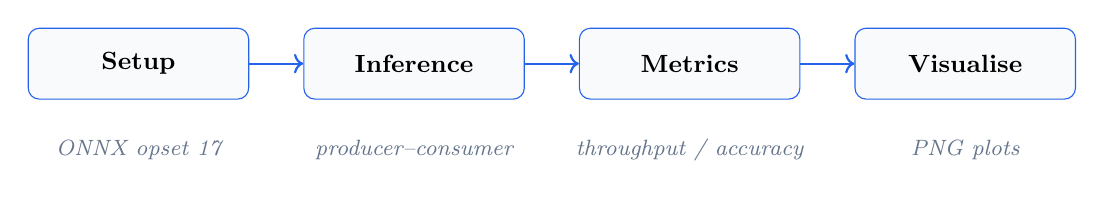
\begin{tikzpicture}[
    box/.style={rectangle, rounded corners=4pt, draw=accent, fill=codebg,
                minimum width=2.8cm, minimum height=0.9cm,
                text centered, font=\small\bfseries},
    arr/.style={->, thick, color=accent},
    note/.style={font=\footnotesize\itshape, color=codegray}
]
    \node[box] (setup) at (0,0)    {Setup};
    \node[box] (inf)   at (3.5,0)  {Inference};
    \node[box] (met)   at (7,0)    {Metrics};
    \node[box] (viz)   at (10.5,0) {Visualise};
    \draw[arr] (setup) -- (inf);
    \draw[arr] (inf)   -- (met);
    \draw[arr] (met)   -- (viz);
    \node[note] at (0,-1.1)    {ONNX opset 17};
    \node[note] at (3.5,-1.1)  {producer--consumer};
    \node[note] at (7,-1.1)    {throughput / accuracy};
    \node[note] at (10.5,-1.1) {PNG plots};
\end{tikzpicture}
\caption{Shared four-stage pipeline common to all three methodologies.}
\label{fig:pipeline_overview}
\end{figure}

\subsection{Model Zoo}

Six ONNX models are evaluated across all methodologies.
Table~\ref{tab:model_zoo} summarises their characteristics.

\begin{table}[H]
\centering
\caption{Model registry and characterisation.}
\label{tab:model_zoo}
\begin{tabular}{lcccccc}
\toprule
\textbf{Model} & \textbf{Input} & \textbf{Classes} & \textbf{Task}
    & \textbf{Source} & \textbf{Min~MB} & \textbf{Top-1} \\
\midrule
ResNet50-v1.5       & $224^2$ & 1000 & cls & torchvision & 90  & $\approx76\%$ \\
MobileNetV2         & $224^2$ & 1000 & cls & torchvision & 12  & $\approx72\%$ \\
MobileNetV3-Small   & $224^2$ & 1000 & cls & torchvision &  8  & $\approx67\%$ \\
MobileNetV1-1.0     & $224^2$ & 1000 & cls & timm        & 14  & $\approx71\%$ \\
EfficientNet-Lite0  & $224^2$ & 1000 & cls & timm        & 15  & $\approx74\%$ \\
SSD-MBv2-backbone   & $300^2$ &  --- & det & torchvision & 10  & N/A \\
\bottomrule
\end{tabular}
\end{table}

\noindent\textbf{timm dependency.}\quad Only \texttt{MobileNetV1} and
\texttt{EfficientNet-Lite0} require the \texttt{timm} library
(\texttt{pip install timm}). All other models depend only on \texttt{torch},
\texttt{torchvision}, \texttt{onnxruntime}, \texttt{numpy}, and
\texttt{pillow}.

\subsection{Dataset Construction}

\subsubsection{Tiny-ImageNet-200 Validation Set}

Tiny-ImageNet-200 is a 200-class subset of ImageNet distributed by Stanford
CS231n~\cite{ref:tiny-imagenet}. The validation partition contains 10\,000
JPEG images ($64\times64$ pixels, 50 per class), annotated with WordNet~IDs
(WNIDs). A handcrafted lookup table $\phi$ maps each WNID to its canonical
ImageNet-1k class index (0--999):
\begin{equation}
    \phi : \text{WNID} \rightarrow \{0, \ldots, 999\} \subset \mathbb{Z}
    \label{eq:wnid}
\end{equation}
All 10\,000 validation images are selected with a fixed random seed
(\texttt{seed=42}). The archive ($\approx$236~MB) is cached locally so that
subsequent runs skip the download.

\subsubsection{Preprocessing Pipeline}
\label{sec:preproc_pipeline}

The models were pre-trained on full ImageNet at $224\times224$ pixels. Since
Tiny-ImageNet images are natively $64\times64$, a three-step preprocessing
pipeline is applied identically across all inference paths:

\begin{figure}[H]
\centering
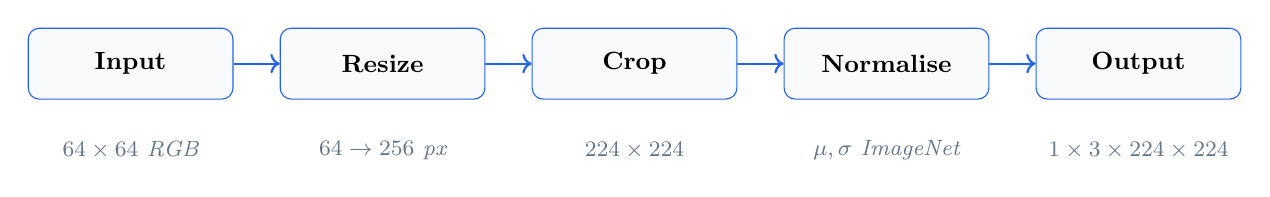
\begin{tikzpicture}[
    box/.style={rectangle, rounded corners=4pt, draw=accent, fill=codebg,
                minimum width=2.6cm, minimum height=0.9cm,
                text centered, font=\small\bfseries},
    arr/.style={->, thick, color=accent},
    note/.style={font=\footnotesize\itshape, color=codegray}
]
    \node[box] (inp)  at (0,0)    {Input};
    \node[box] (res)  at (3.2,0)  {Resize};
    \node[box] (crp)  at (6.4,0)  {Crop};
    \node[box] (nrm)  at (9.6,0)  {Normalise};
    \node[box] (out)  at (12.8,0) {Output};
    \draw[arr] (inp) -- (res);
    \draw[arr] (res) -- (crp);
    \draw[arr] (crp) -- (nrm);
    \draw[arr] (nrm) -- (out);
    \node[note] at (0,-1.1)    {$64\times64$ RGB};
    \node[note] at (3.2,-1.1)  {$64\to256$~px};
    \node[note] at (6.4,-1.1)  {$224\times224$};
    \node[note] at (9.6,-1.1)  {$\mu,\sigma$ ImageNet};
    \node[note] at (12.8,-1.1) {$1\times3\times224\times224$};
\end{tikzpicture}
\caption{Tiny-ImageNet preprocessing pipeline applied identically on every
inference path.}
\label{fig:preproc_pipeline}
\end{figure}

\begin{enumerate}[itemsep=1pt, topsep=3pt]
    \item \textbf{Bilinear resize:} The image is resized so that its shorter
          dimension equals 256~px, preserving aspect ratio. PIL
          \texttt{BILINEAR} interpolation is used, consistent with the
          standard ImageNet evaluation protocol.

    \item \textbf{Centre crop to $224\times224$:} A $224\times224$ region is
          extracted from the centre of the $256\times256$ intermediate. The
          crop offsets are:
          \begin{equation}
              \text{left} = \lfloor(W-224)/2\rfloor,\quad
              \text{top}  = \lfloor(H-224)/2\rfloor
          \end{equation}
          where $W$ and $H$ are the width and height of the resized image.

    \item \textbf{Normalisation:} Each pixel value is scaled to $[0,1]$ by
          dividing by 255, then standardised channel-wise:
          \begin{equation}
              x_c^{\prime} = \frac{x_c/255 - \mu_c}{\sigma_c},\quad
              c\in\{R,G,B\},\quad
              \mu=[0.485,0.456,0.406],\quad
              \sigma=[0.229,0.224,0.225]
          \end{equation}
\end{enumerate}

The output is a \texttt{float32} NumPy array of shape $[1,3,224,224]$,
memory footprint $\approx0.60$~MB. This tensor's DMA transfer from LPDDR4
into NPU SRAM constitutes the fixed overhead $\Delta_{\text{DMA}}=0.18$~ms
in the NPU simulation (Section~\ref{sec:m2_npu_sim}).

\paragraph{Impact on accuracy.}
Upsampling from $64\times64$ to $224\times224$ introduces bilinear blur not
present during training. Top-1 accuracy is consequently 16\%--31\% versus the
69\%--80\% these models achieve on genuine ImageNet data. Accuracy is treated
as a \emph{sanity check}: values well above the $\approx0.1\%$ random
baseline confirm correct model loading, label remapping, and preprocessing
integrity. Latency measurements — the primary benchmark output — are
unaffected by the resolution mismatch.

% =============================================================================
\section{Methodology 1: x86 CPU Baseline}
\label{sec:m1_design}
% =============================================================================

\subsection{Overview}

Methodology~1 establishes a reproducible performance baseline by executing
unmodified \texttt{float32} ONNX models on an AMD Ryzen~5 5600H using ONNX
Runtime's \texttt{CPUExecutionProvider}. This serves two purposes: (1)
confirming that pretrained weights are correctly loaded and characterising
accuracy under the Tiny-ImageNet resolution mismatch, and (2) providing
reference latency measurements for relative comparison with the
simulation-based methodologies.

\subsection{ONNX Runtime Session Configuration}

Sessions are created with full graph optimisation enabled. The number of
intra-op and inter-op threads is set to~0 (auto), allowing ONNX Runtime to
utilise all available physical cores for maximum parallelism.

\begin{lstlisting}[language=Python,
    caption={ONNX Runtime session creation with full graph optimisation.}]
opts = ort.SessionOptions()
opts.intra_op_num_threads     = 0   # auto = all physical cores
opts.inter_op_num_threads     = 0
opts.graph_optimization_level = ort.GraphOptimizationLevel.ORT_ENABLE_ALL
opts.enable_profiling         = False

session = ort.InferenceSession(
    model_path,
    sess_options=opts,
    providers=["CPUExecutionProvider"]
)
\end{lstlisting}

\subsection{Producer--Consumer Pipeline}

To prevent preprocessing from inflating inference timing, a
producer--consumer architecture decouples JPEG decode/resize from ONNX
session execution:

\begin{itemize}[itemsep=1pt, topsep=3pt]
    \item \textbf{Producer:} A \texttt{ThreadPoolExecutor} with 4 workers
          preprocesses images and submits ready tensors to a bounded queue
          (capacity 32). The producer maintains the original image index,
          preserving the link between image, tensor, and ground-truth label.
    \item \textbf{Consumer:} The main thread pulls pre-built tensors from the
          queue and calls \texttt{session.run()} sequentially, recording
          per-inference latency.
\end{itemize}

\begin{figure}[H]
\centering
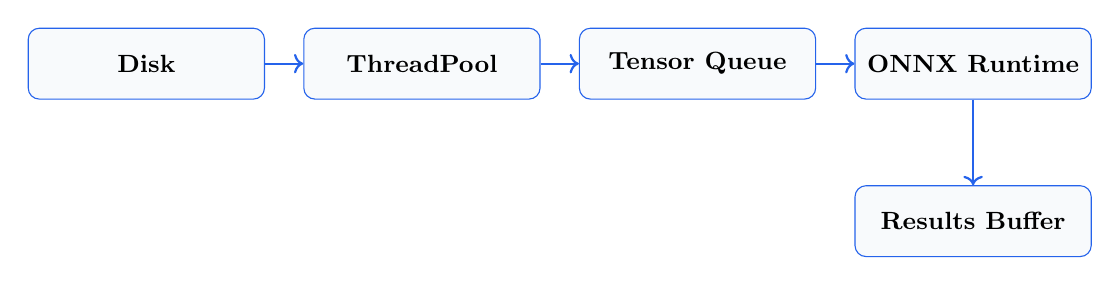
\begin{tikzpicture}[
    box/.style={rectangle, rounded corners=4pt, draw=accent, fill=codebg,
                minimum width=3.0cm, minimum height=0.9cm,
                text centered, font=\small\bfseries},
    arr/.style={->, thick, color=accent}
]
    \node[box] (disk)  at (0,0)   {Disk};
    \node[box] (pool)  at (3.5,0) {ThreadPool};
    \node[box] (queue) at (7,0)   {Tensor Queue};
    \node[box] (ort)   at (10.5,0){ONNX Runtime};
    \node[box] (out)   at (10.5,-2){Results Buffer};
    \draw[arr] (disk)  -- (pool);
    \draw[arr] (pool)  -- (queue);
    \draw[arr] (queue) -- (ort);
    \draw[arr] (ort)   -- (out);
\end{tikzpicture}
\caption{Producer--consumer inference pipeline for Methodology~1.}
\label{fig:m1_pipeline}
\end{figure}

\subsection{Timing Isolation}

Only the \texttt{session.run()} call is timed using
\texttt{time.perf\_counter()}:
\begin{equation}
    t_{\text{inf},i} = t_1 - t_0,\quad
    t_0 = \texttt{perf\_counter()\ before},\quad
    t_1 = \texttt{perf\_counter()\ after}
\end{equation}
Preprocessing time is recorded separately as an overlapped cost and does not
contribute to the inference latency histogram.

\subsection{Warm-up Protocol}

Five initial inference calls are executed before timing begins and excluded
from all latency statistics. This protocol: (1) completes ONNX Runtime JIT
compilation, (2) warms CPU instruction caches and the TLB, and (3) initialises
BLAS thread pools and numerical libraries.

\subsection{Inference Algorithm}

\begin{algorithm}[H]
\caption{Methodology~1 Baseline Inference Benchmark}
\label{alg:m1_inference}
\begin{algorithmic}[1]
\Require Model $\mathcal{M}$, dataset $\mathcal{D}=\{(x_i,y_i)\}_{i=0}^{N-1}$,
         $W=5$, $Q=16$, $P=4$
\Ensure Latency vector $\mathbf{L}\in\mathbb{R}^N$, accuracy $A$
\State Create ORT session $S$ with \texttt{ORT\_ENABLE\_ALL}
\For{$w=1\ldots W$}
    \State $S.\texttt{run}(\texttt{preprocess}(x_0))$ \Comment{warm-up, discarded}
\EndFor
\State Start producer with $P$ workers, queue capacity $2Q$
\For{$i=0\ldots N-1$}
    \State $(i',\hat{x},t_\text{pp})\gets\mathcal{Q}.\texttt{get}()$
    \State $t_0\gets\texttt{perf\_counter}()$
    \State $\hat{y}\gets S.\texttt{run}(\hat{x})$
    \State $t_1\gets\texttt{perf\_counter}()$
    \State $L_{i'}\gets(t_1-t_0)\times1000$ \Comment{ms}
    \If{task $=$ \texttt{cls}}
        \State $\text{correct}_{i'}\gets\mathbf{1}[\arg\max\hat{y}=y_{i'}]$
    \EndIf
\EndFor
\State $A\gets\frac{1}{N}\sum\text{correct}_i\times100$ \textbf{if} cls \textbf{else} \textsc{None}
\State \Return $\mathbf{L}$, $A$
\end{algorithmic}
\end{algorithm}

\subsection{Statistical Metrics}

For each model, the latency vector $\mathbf{L}=(L_0,\ldots,L_{N-1})$ in
milliseconds yields:

\begin{itemize}[itemsep=1pt, topsep=3pt]
    \item \textbf{Mean:} $\bar{L}=\frac{1}{N}\sum L_i$
    \item \textbf{Median (p50):} $L_{0.50}$, the typical latency
    \item \textbf{p95:} $L_{0.95}$, the SLA tail
    \item \textbf{p99:} $L_{0.99}$, the strict tail used in MLPerf
    \item \textbf{Std:} $\sigma=\sqrt{\frac{1}{N}\sum(L_i-\bar{L})^2}$
    \item \textbf{IQR:} $L_{0.75}-L_{0.25}$
    \item \textbf{Throughput:} $T=1000/\bar{L}$ img/s
    \item \textbf{CV:} $\sigma/\bar{L}$; $<0.10$ stable, $\in[0.10,0.30)$
          moderate jitter, $\geq0.30$ high jitter
\end{itemize}

\subsection{Experimental Setup}

\begin{table}[H]
\centering
\caption{Host hardware and software environment for Methodology~1.}
\label{tab:m1_env}
\begin{tabular}{ll}
\toprule
\textbf{Parameter} & \textbf{Value} \\
\midrule
Hardware             & x86-64 AMD Ryzen~5 5600H \\
Runtime              & ONNX Runtime \texttt{CPUExecutionProvider} \\
Batch size           & 1 (sequential) \\
Warm-up runs         & 5 (excluded from timing) \\
Preprocessing workers& 4 threads (\texttt{ThreadPoolExecutor}) \\
Queue depth          & 32 tensors \\
Dataset              & Tiny-ImageNet-200 validation, $N=10{,}000$ \\
Label space          & ImageNet-1k (0--999) \\
\bottomrule
\end{tabular}
\end{table}

\subsection{Results}

\subsubsection{Latency and Throughput}

\begin{table}[H]
\centering
\caption{Latency and throughput results --- x86 CPU baseline.}
\label{tab:m1_results_lat}
\resizebox{\textwidth}{!}{%
\begin{tabular}{lcccccccc}
\toprule
\textbf{Model} & \textbf{Task} & \textbf{$\bar{L}$ (ms)} & \textbf{p50}
    & \textbf{p95} & \textbf{p99} & \textbf{$\sigma$} & \textbf{CV}
    & \textbf{img/s} \\
\midrule
ResNet50-v1.5       & cls & 22.74 & 19.24 & 41.37 & 66.39 & 9.52 & 0.419 & 43.98 \\
MobileNetV2         & cls &  4.58 &  4.15 &  7.68 & 11.82 & 1.96 & 0.429 & 218.52 \\
MobileNetV3-Small   & cls &  3.45 &  3.43 &  5.32 &  7.35 & 1.20 & 0.348 & 289.89 \\
MobileNetV1-1.0     & cls &  6.05 &  5.20 & 11.06 & 17.89 & 2.80 & 0.464 & 165.39 \\
EfficientNet-Lite0  & cls &  5.45 &  4.85 &  9.31 & 14.37 & 2.39 & 0.438 & 183.43 \\
SSD-MBv2-backbone   & det &  7.87 &  6.81 & 13.51 & 24.72 & 3.69 & 0.469 & 127.01 \\
\bottomrule
\end{tabular}}
\end{table}

\subsubsection{Visualisation Suite}

\paragraph{Latency over time.}
Per-image latency trace overlaid with mean $\bar{L}$, p95, and $\pm1\sigma$
band. A flat trace indicates thermal and frequency stability; a rising trend
indicates thermal throttling; spikes indicate OS scheduling jitter.

\subsection{Latency Distribution: Histogram and KDE Visualisation}

Combined histogram and Gaussian KDE with Scott's bandwidth rule
$h = n^{-1/5}\cdot\sigma$. Mean and p95 are marked with dashed/dotted
vertical lines. A narrow tall peak indicates consistent performance; a heavy
right tail signals occasional stalls.

\begin{figure}[H]
    \centering
    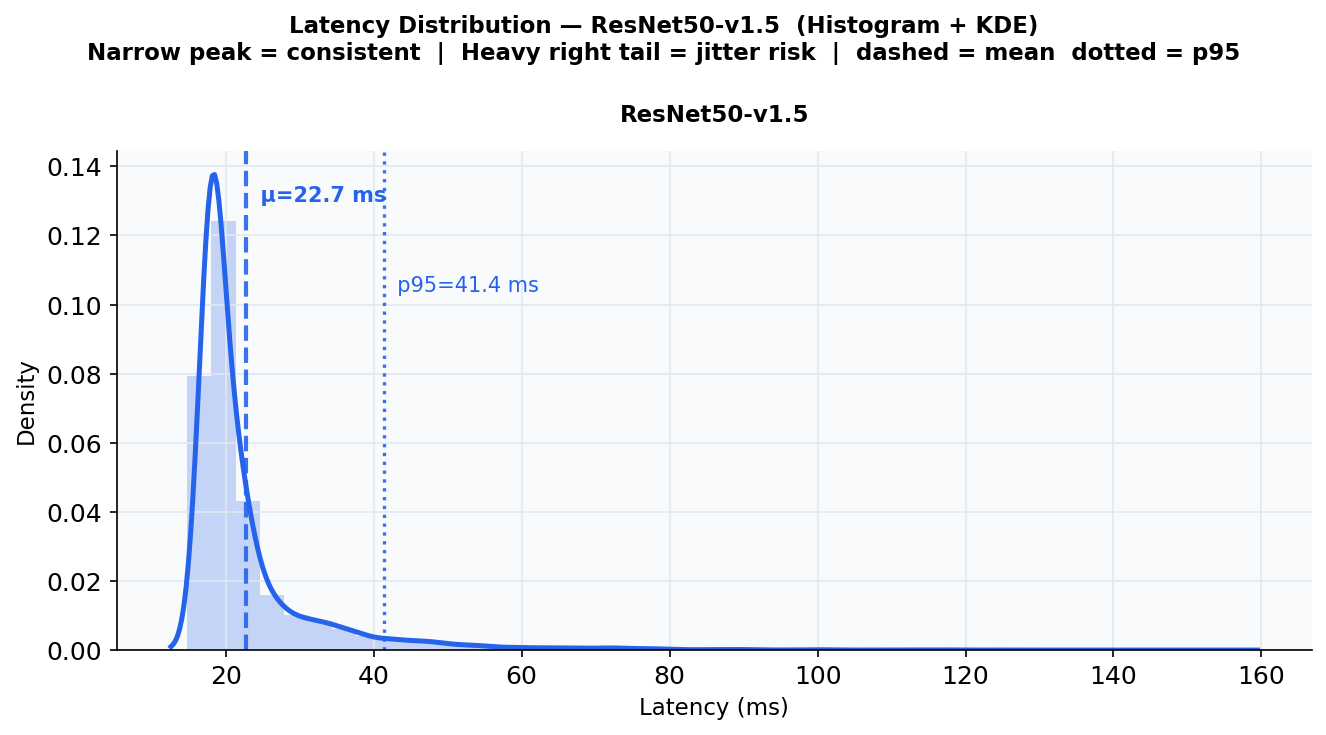
\includegraphics[width=\textwidth]{img/pics updated hiararchy pfe/Latency Distribution/1-242-1.png}
    \caption{Latency distribution --- ResNet50-v1.5.}
    \label{fig:m1_hist_resnet50}
\end{figure}

\begin{figure}[H]
    \centering
    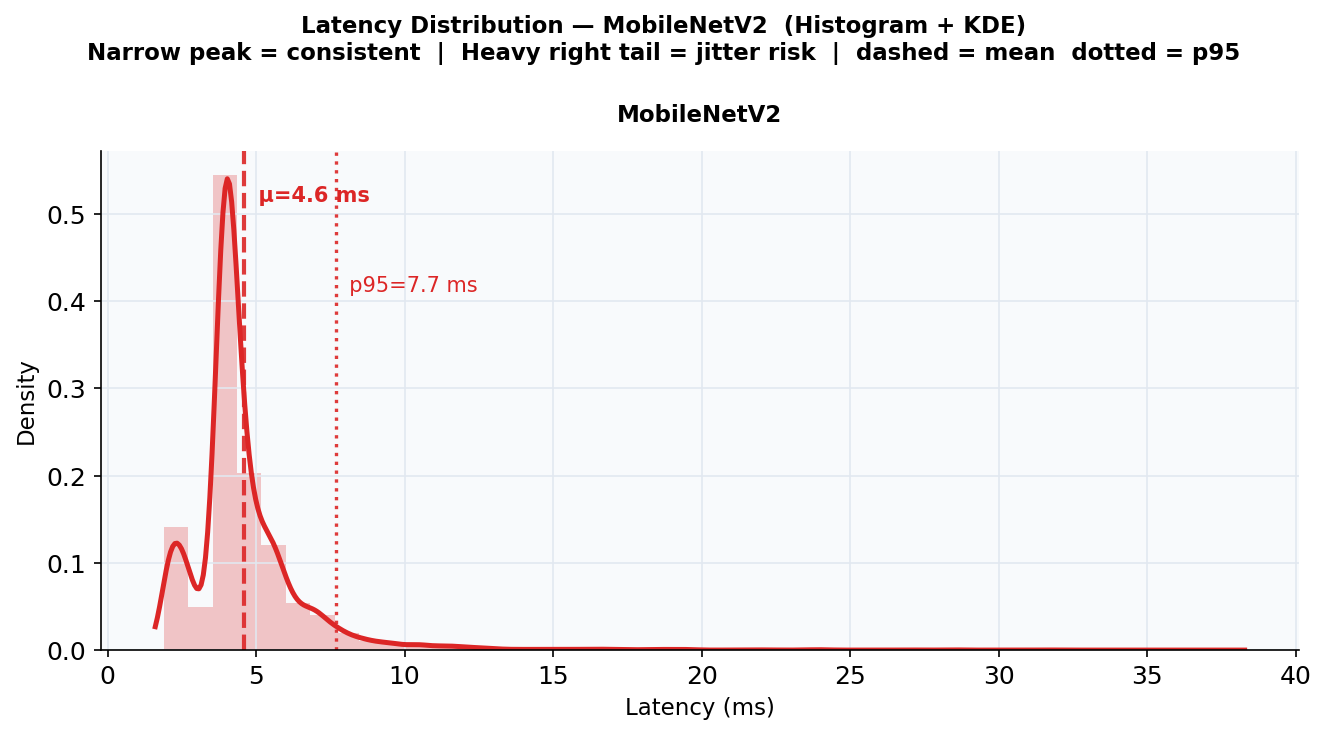
\includegraphics[width=\textwidth]{img/pics updated hiararchy pfe/Latency Distribution/1-242-2.png}
    \caption{Latency distribution --- MobileNetV2.}
    \label{fig:m1_hist_mbv2}
\end{figure}

\begin{figure}[H]
    \centering
    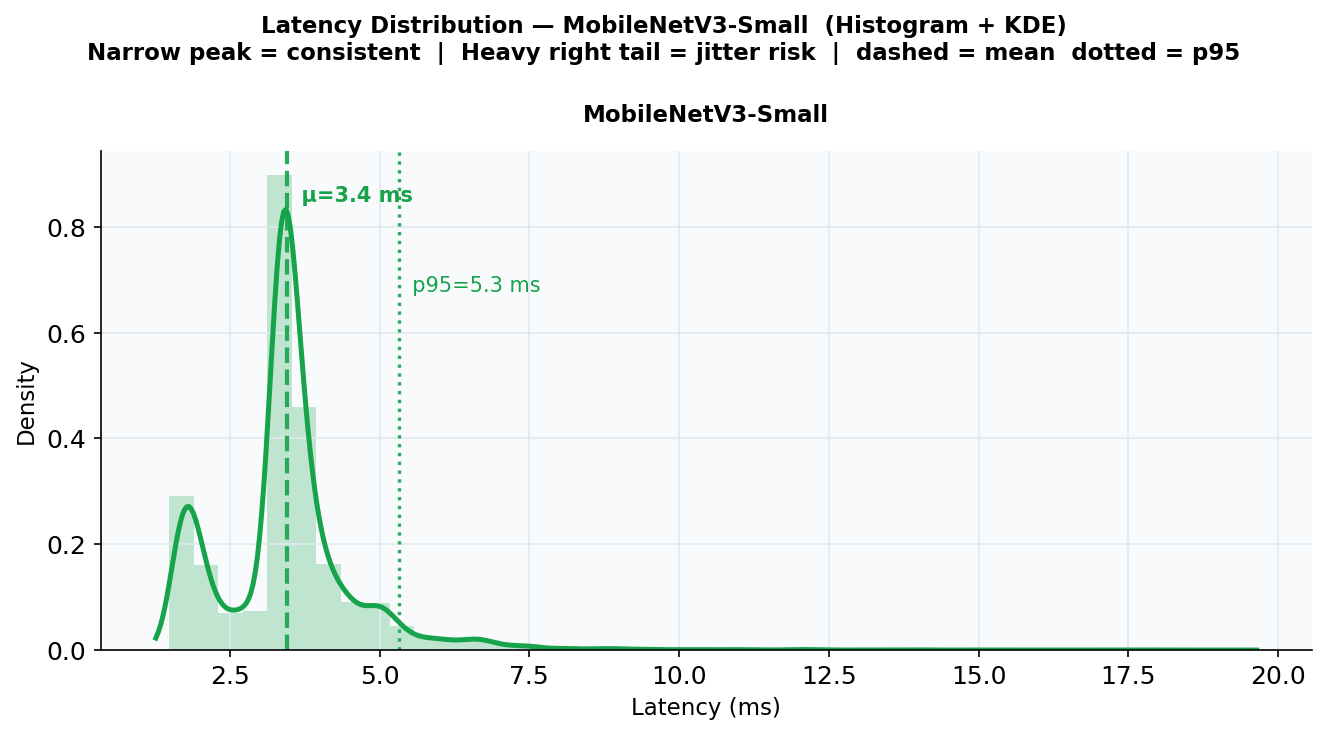
\includegraphics[width=\textwidth]{img/pics updated hiararchy pfe/Latency Distribution/1-242-3.png}
    \caption{Latency distribution --- MobileNetV3-Small.}
    \label{fig:m1_hist_mbv3small}
\end{figure}

\begin{figure}[H]
    \centering
    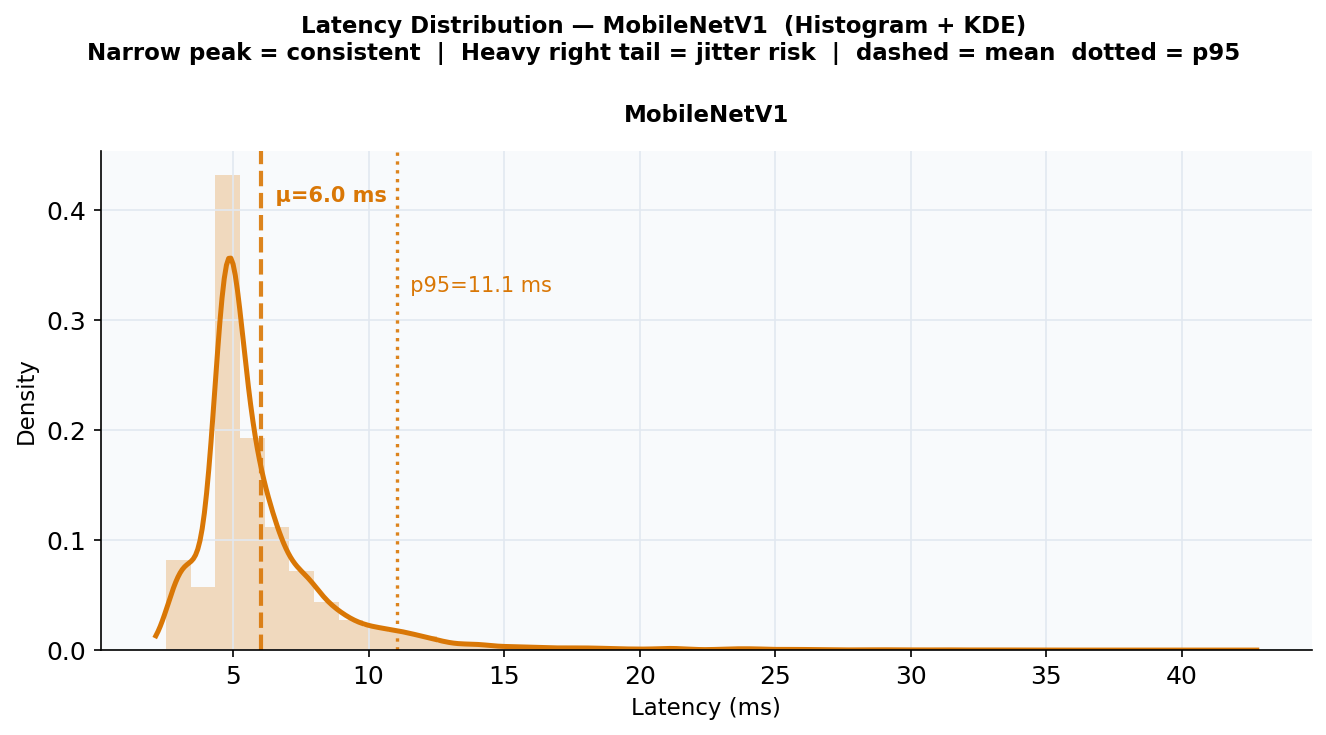
\includegraphics[width=\textwidth]{img/pics updated hiararchy pfe/Latency Distribution/1-242-4.png}
    \caption{Latency distribution --- MobileNetV1.}
    \label{fig:m1_hist_mbv1}
\end{figure}

\begin{figure}[H]
    \centering
    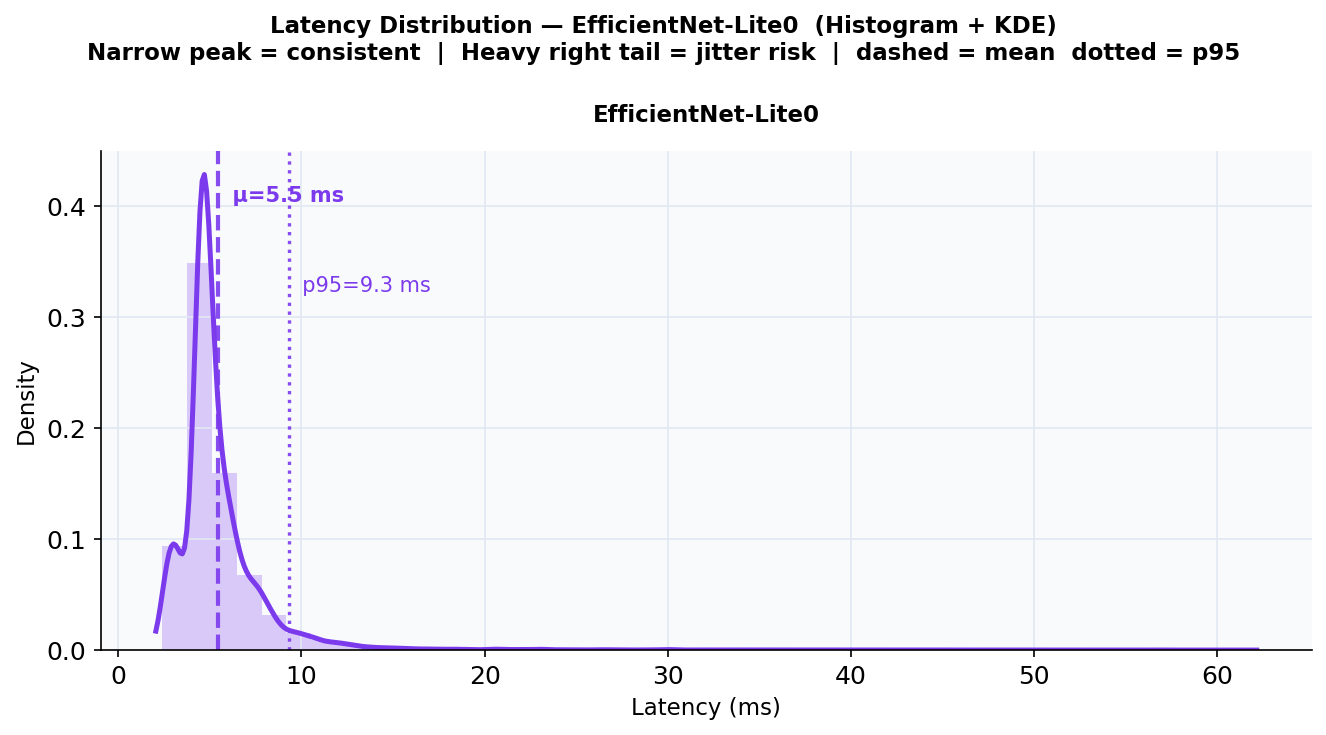
\includegraphics[width=\textwidth]{img/pics updated hiararchy pfe/Latency Distribution/1-242-5.png}
    \caption{Latency distribution --- EfficientNet-Lite0.}
    \label{fig:m1_hist_effnet}
\end{figure}

\begin{figure}[H]
    \centering
    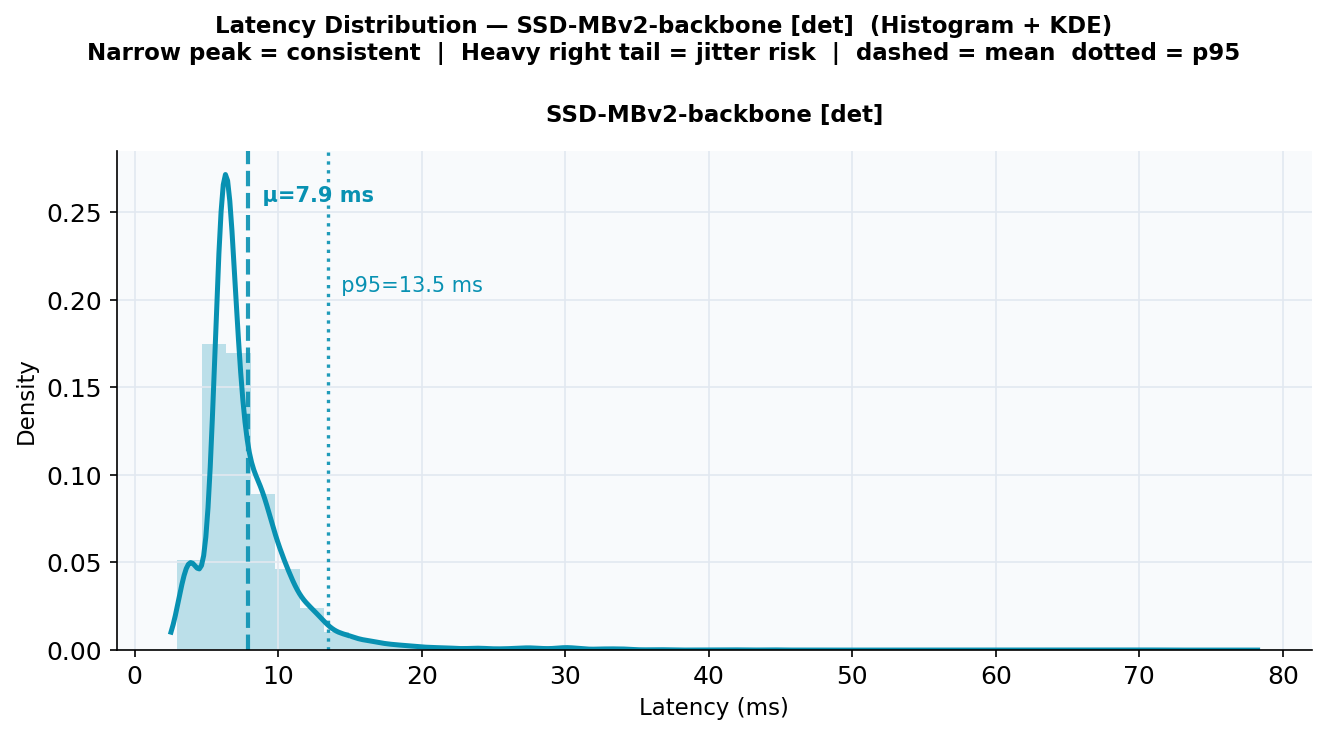
\includegraphics[width=\textwidth]{img/pics updated hiararchy pfe/Latency Distribution/1-242-6.png}
    \caption{Latency distribution --- SSD-MBv2-backbone.}
    \label{fig:m1_hist_ssd}
\end{figure}
\paragraph{Latency distribution (histogram + KDE).}
Combined histogram and Gaussian KDE with Scott's bandwidth rule
$h=n^{-1/5}\cdot\sigma$. Mean and p95 are marked with dashed/dotted vertical
lines. A narrow tall peak indicates consistent performance; a heavy right tail
signals occasional stalls.

% ---- PLACEHOLDER: Histogram+KDE plots (Methodology 1) ----
% \begin{figure}[H]
%     \centering
%     \includegraphics[width=\textwidth]{vis/m1_hist_resnet50.png}
%     \caption{Latency distribution --- ResNet50-v1.5.}
%     \label{fig:m1_hist_resnet}
% \end{figure}
% ... (repeat for the remaining five models)

\paragraph{Preprocessing vs.\ inference time breakdown.}

% ---- PLACEHOLDER: Time breakdown stacked bar (Methodology 1) ----
% \begin{figure}[H]
%     \centering
%     \includegraphics[width=\textwidth]{vis/m1_time_breakdown.png}
%     \caption{Preprocessing vs.\ inference time breakdown (x86 CPU baseline).}
%     \label{fig:m1_breakdown}
% \end{figure}

\paragraph{Accuracy--latency Pareto scatter.}
The Pareto frontier connects all models not dominated by any other candidate.
A model is dominated if there exists another with simultaneously higher
accuracy \emph{and} lower latency. Accuracy figures are indicative
(Tiny-ImageNet upsampling degrades all models uniformly), but relative
positions and the frontier are valid for comparative analysis.

% ---- PLACEHOLDER: Pareto scatter (Methodology 1) ----
% \begin{figure}[H]
%     \centering
%     \includegraphics[width=\textwidth]{vis/m1_pareto.png}
%     \caption{Accuracy--latency Pareto scatter for classification models
%              (x86 CPU baseline).}
%     \label{fig:m1_pareto}
% \end{figure}

% =============================================================================
\section{Methodology 2: Physics-Based ARM and NPU Simulation}
\label{sec:m2_design}
% =============================================================================

\subsection{Overview and Motivation}

Methodology~2 extends the x86 baseline by simulating what inference would look
like on the NXP i.MX~8M~Plus embedded board before physical hardware is
available. The simulation executes entirely on the host x86 machine and
produces three latency estimates for every inference call — a \emph{tri-path}
execution:

\begin{description}[itemsep=1pt, topsep=3pt]
    \item[\textbf{Path~A — x86 Host (measured):}] The actual wall-clock time
          of a real ONNX Runtime forward pass on the host CPU.
    \item[\textbf{Path~B — ARM Cortex-A53 CPU (simulated):}] An estimate of
          how long the same model would take on the ARM Cortex-A53 processor,
          derived by applying a sequence of six physical effects to the real
          x86 measurement.
    \item[\textbf{Path~C — Vivante GC7000UltraLite NPU (simulated):}] An
          estimate of NPU inference latency, anchored to a calibration mean
          and independent of per-image x86 measurements.
\end{description}

Accuracy is identical across all three paths because the logits come from a
single real ONNX Runtime forward pass. Only \emph{latency} differs.

\subsection{Target Hardware Specification}

\begin{table}[H]
\centering
\caption{NXP i.MX~8M~Plus hardware specification targeted by the simulation.}
\label{tab:imx8_spec}
\begin{tabular}{ll}
\toprule
\textbf{Component} & \textbf{Specification} \\
\midrule
SoC         & NXP i.MX~8M~Plus \\
CPU cluster & 4$\times$ ARM Cortex-A53 @ 1.8~GHz \\
SIMD        & ARMv8-A NEON (128-bit vector width) \\
NPU         & Vivante GC7000UltraLite, 2.3~TOPS (INT8) \\
RAM         & 4~GB LPDDR4 @ 25.6~GB/s peak \\
OS          & Yocto Linux (single-user embedded profile) \\
\bottomrule
\end{tabular}
\end{table}

\subsection{Tri-Path Architecture and Two-Pass Strategy}

A circular dependency exists: the NPU simulator needs the ARM CPU mean latency
before it can set its base, but that mean is only known after the ARM CPU
simulator has processed images. The implementation resolves this with a
two-pass approach:

\begin{enumerate}[itemsep=1pt, topsep=3pt]
    \item \textbf{Calibration pass (200 images):} Real ONNX Runtime forward
          passes yield $\bar{L}_{\text{x86}}^{\text{calib}}$. The ARM CPU
          calibration mean is:
          \begin{equation}
              \bar{L}_{\text{ARM}}^{\text{calib}}
              = \bar{L}_{\text{x86}}^{\text{calib}} \times s_{\text{cpu}}
          \end{equation}
          The NPU base latency is then fixed as:
          \begin{equation}
              L_{\text{NPU}}^{\text{base}}
              = \bar{L}_{\text{ARM}}^{\text{calib}} \times s_{\text{NPU}}
          \end{equation}

    \item \textbf{Full benchmark pass ($N$ images):} For every image, one
          real forward pass produces $L_i^{\text{x86}}$ and output logits.
          Path~B receives $L_i^{\text{x86}}$ and applies the six-effect
          physics model; Path~C takes no per-image input and estimates NPU
          latency analytically.
\end{enumerate}

\subsection{Path B: ARM Cortex-A53 CPU Simulator}
\label{sec:m2_arm_cpu_sim}

The \texttt{ARMCPUSimulator} converts each real x86 latency into an estimated
ARM Cortex-A53 latency by applying six physical effects in sequence.

\subsubsection{The Six Effects}

\begin{enumerate}[itemsep=1pt, topsep=3pt]
    \item \textbf{Architecture scaling (Effect~1):} $L \gets L_i^{\text{x86}}
          \times s_{\text{cpu}}$ ($3.4$--$4.5\times$) captures the throughput
          gap between ARM NEON (128-bit, in-order) and x86 AVX2 (256-bit,
          out-of-order).
    \item \textbf{NEON execution jitter (Effect~2):}
          $\epsilon\sim\mathcal{N}(0,(\mathrm{CV}_j\cdot L)^2)$, floor at
          $0.5L$.
    \item \textbf{Cold-cache warm-up penalty (Effect~3):} First
          $N_{\text{warmup}}$ images pay a linearly decaying penalty $p_w$.
    \item \textbf{Thermal drift (Effect~4):} After $N_{\text{thermal}}$ images,
          latency increases linearly by up to $2\delta_T$.
    \item \textbf{LPDDR4 memory bandwidth spike (Effect~5):} With probability
          $p_{\text{mem}}=4\%$, latency is multiplied by $f_{\text{mem}}=1.35$.
    \item \textbf{QEMU TCG timing noise (Effect~6):}
          $L \gets L\times(1+\mathcal{U}(-c_{\text{TCG}},c_{\text{TCG}}))$,
          default $\pm3\%$.
\end{enumerate}

Output is clamped to a minimum of 0.1~ms.

\subsubsection{ARM CPU Simulation Algorithm}

\begin{algorithm}[H]
\caption{ARM Cortex-A53 CPU Latency Simulation
         (\texttt{ARMCPUSimulator.simulate()})}
\label{alg:m2_arm_cpu_sim}
\begin{algorithmic}[1]
\Require $L_i^{\text{x86}}$, internal counter $i$, per-model and global
         simulation parameters
\Ensure $L_i^{\text{CPU}}$ (simulated ARM latency, ms)
\State $i\gets\texttt{n\_images}$;\quad$\texttt{n\_images}\gets\texttt{n\_images}+1$
\State $L\gets L_i^{\text{x86}}\times s_{\text{cpu}}$
       \Comment{Effect 1: Architecture scaling}
\State $\epsilon\sim\mathcal{N}(0,(\mathrm{CV}_j\cdot L)^2)$;\quad
       $L\gets\max(0.5L,\,L+\epsilon)$
       \Comment{Effect 2: NEON jitter}
\If{$i<N_{\text{warmup}}$}
    \State $L\gets L\times(1+p_w\cdot(1-i/N_{\text{warmup}}))$
           \Comment{Effect 3: Cold-cache penalty}
\EndIf
\If{$i>N_{\text{thermal}}$}
    \State $\alpha\gets\min(1,(i-N_{\text{thermal}})/\max(1,10000-N_{\text{thermal}}))$
    \State $L\gets L\times(1+2\delta_T\alpha)$
           \Comment{Effect 4: Thermal drift}
\EndIf
\If{$u\sim\mathcal{U}(0,1)<p_{\text{mem}}$}
    \State $L\gets L\times f_{\text{mem}}$
           \Comment{Effect 5: Memory bandwidth spike}
\EndIf
\State $L\gets L\times(1+\mathcal{U}(-c_{\text{TCG}},c_{\text{TCG}}))$
       \Comment{Effect 6: QEMU TCG noise}
\State\Return $\max(0.1,L)$
\end{algorithmic}
\end{algorithm}

\subsubsection{Python Implementation}

\begin{lstlisting}[language=Python,
    caption={\texttt{ARMCPUSimulator.simulate()} from
             \texttt{inference\_qemu.py}.}]
def simulate(self, x86_lat_ms: float) -> float:
    i = self.n_images
    self.n_images += 1

    lat = x86_lat_ms * self.cpu_scale                          # Effect 1
    lat = max(lat * 0.5,
              lat + self.rng.normal(0.0, self.jitter_cv * lat))# Effect 2
    if i < self.n_warmup:
        decay = 1.0 - (i / self.n_warmup)
        lat  *= (1.0 + self.warmup_penalty * decay)            # Effect 3
    if i > self.n_thermal:
        progress = min(1.0, (i - self.n_thermal) /
                       max(1, 10000 - self.n_thermal))
        lat *= (1.0 + self.thermal_drift * 2.0 * progress)    # Effect 4
    if self.rng.random() < self.mem_prob:
        lat *= self.mem_factor                                 # Effect 5
    lat *= (1.0 + self.rng.uniform(-self.tcg_noise_cv,
                                    self.tcg_noise_cv))        # Effect 6
    return max(0.1, lat)
\end{lstlisting}

\subsection{Path C: Vivante GC7000UltraLite NPU Simulator}
\label{sec:m2_npu_sim}

The \texttt{ARMNPUSimulator} uses a single fixed base latency
$L_{\text{NPU}}^{\text{base}}$ and applies six independent effects.

\subsubsection{NPU Simulation Algorithm}

\begin{algorithm}[H]
\caption{Vivante GC7000UltraLite NPU Latency Simulation
         (\texttt{ARMNPUSimulator.simulate()})}
\label{alg:m2_npu_sim}
\begin{algorithmic}[1]
\Require $L_{\text{NPU}}^{\text{base}}$, $\rho_{\text{SE}}$,
         $\Delta_{\text{quant}}$, $\Delta_{\text{DMA}}$,
         $\text{CV}_{\text{NPU}}=0.030$, $p_{\text{mem}}=0.04$,
         $f_{\text{mem}}=1.35$
\Ensure $L^{\text{NPU}}$ (ms)
\State $L\gets L_{\text{NPU}}^{\text{base}}$
       \Comment{Effect 1: Base throughput}
\State $L\gets L\times\rho_{\text{SE}}$
       \Comment{Effect 2: SE-block penalty}
\State $L\gets L+\Delta_{\text{quant}}$
       \Comment{Effect 3: INT8 dequantisation overhead}
\State $L\gets L+\Delta_{\text{DMA}}$
       \Comment{Effect 4: DMA input staging}
\State $\epsilon\sim\mathcal{N}(0,(\text{CV}_{\text{NPU}}\cdot L)^2)$;\quad
       $L\gets\max(0.7L,\,L+\epsilon)$
       \Comment{Effect 5: Small random jitter}
\If{$u\sim\mathcal{U}(0,1)<p_{\text{mem}}$}
    \State $L\gets L\times f_{\text{mem}}$
           \Comment{Effect 6: Shared memory bandwidth spike}
\EndIf
\State\Return $\max(0.05,L)$
\end{algorithmic}
\end{algorithm}

Effects deliberately excluded from the NPU model: thermal drift (NPU has its
own power domain), cache warm-up (256~KB SRAM holds all model weights), and
QEMU TCG noise (latency is computed analytically).

\subsection{Per-Model Parameter Justification}

\begin{table}[H]
\centering
\caption{Per-model simulation parameters.}
\label{tab:m2_per_model_config}
\begin{tabular}{lcccc}
\toprule
\textbf{Model} & \textbf{Task}
    & \textbf{CPU scale $s_{\text{cpu}}$}
    & \textbf{NPU scale $s_{\text{NPU}}$}
    & \textbf{Jitter CV} \\
\midrule
ResNet50-v1.5       & cls & 4.5 & 0.18           & 0.08 \\
MobileNetV2         & cls & 3.8 & 0.15           & 0.07 \\
MobileNetV3-Small   & cls & 3.6 & 0.20$^\dagger$ & 0.07 \\
MobileNetV1         & cls & 3.4 & 0.12           & 0.06 \\
EfficientNet-Lite0  & cls & 3.9 & 0.14           & 0.07 \\
SSD-MBv2-backbone   & det & 4.1 & 0.16           & 0.10 \\
\bottomrule
\multicolumn{5}{p{0.95\textwidth}}{\footnotesize
$^\dagger$MobileNetV3-Small also carries $\rho_{\text{SE}}=1.08$ applied
multiplicatively inside \texttt{ARMNPUSimulator.simulate()}.}
\end{tabular}
\end{table}

CPU scale factors range from $3.4\times$ (MobileNetV1, memory-bandwidth
limited) to $4.5\times$ (ResNet50-v1.5, compute-limited GEMM). NPU scale
factors range from 0.12 (MobileNetV1, ideal SRAM fit and operator fusion) to
0.20 (MobileNetV3-Small, SE-block memory round-trips). Jitter CV ranges from
0.06 (small model, L1/L2 resident) to 0.10 (SSD with $300\times300$ input
causing continuous L2 overflow).

\subsection{Simulation Results}

\begin{table}[H]
\centering
\caption{Tri-path mean latency comparison (Methodology~2).}
\label{tab:m2_results}
\resizebox{\textwidth}{!}{%
\begin{tabular}{lcccccccc}
\toprule
\textbf{Model} & \textbf{Task}
    & \textbf{x86 ms} & \textbf{ARM ms} & \textbf{NPU ms}
    & \textbf{ARM/x86} & \textbf{NPU/CPU} & \textbf{NPU/x86}
    & \textbf{Acc (\%)} \\
\midrule
ResNet50-v1.5      & cls & 28.6 & 133.7 & 24.1 & $4.68\times$ & $5.56\times$ & $1.19\times$ & 30.6 \\
MobileNetV2        & cls &  5.1 &  19.9 &  3.0 & $3.93\times$ & $6.67\times$ & $1.71\times$ & 22.8 \\
MobileNetV3-Small  & cls &  3.7 &  13.8 &  2.8 & $3.71\times$ & $5.00\times$ & $1.34\times$ & 23.4 \\
MobileNetV1-1.0    & cls &  7.0 &  24.4 &  2.9 & $3.49\times$ & $8.33\times$ & $2.41\times$ & 16.1 \\
EfficientNet-Lite0 & cls &  6.2 &  24.9 &  3.5 & $4.02\times$ & $7.14\times$ & $1.78\times$ & 31.7 \\
SSD-MBv2-backbone  & det & 10.2 &  43.5 &  --- & $4.28\times$ &          --- &          --- & N/A  \\
\bottomrule
\end{tabular}}
\end{table}

\subsection{Visualisation Suite}
\label{sec:m2_vis}
\subsection{Latency Distribution: Histogram and KDE Visualisation}

Combined histogram and Gaussian KDE with Scott's bandwidth rule
$h = n^{-1/5}\cdot\sigma$. Mean and p95 are marked with dashed/dotted
vertical lines. A narrow tall peak indicates consistent performance; a heavy
right tail signals occasional stalls.

% All figures placed on dedicated float pages to avoid blocking the text
\begin{figure}[p]
    \centering
    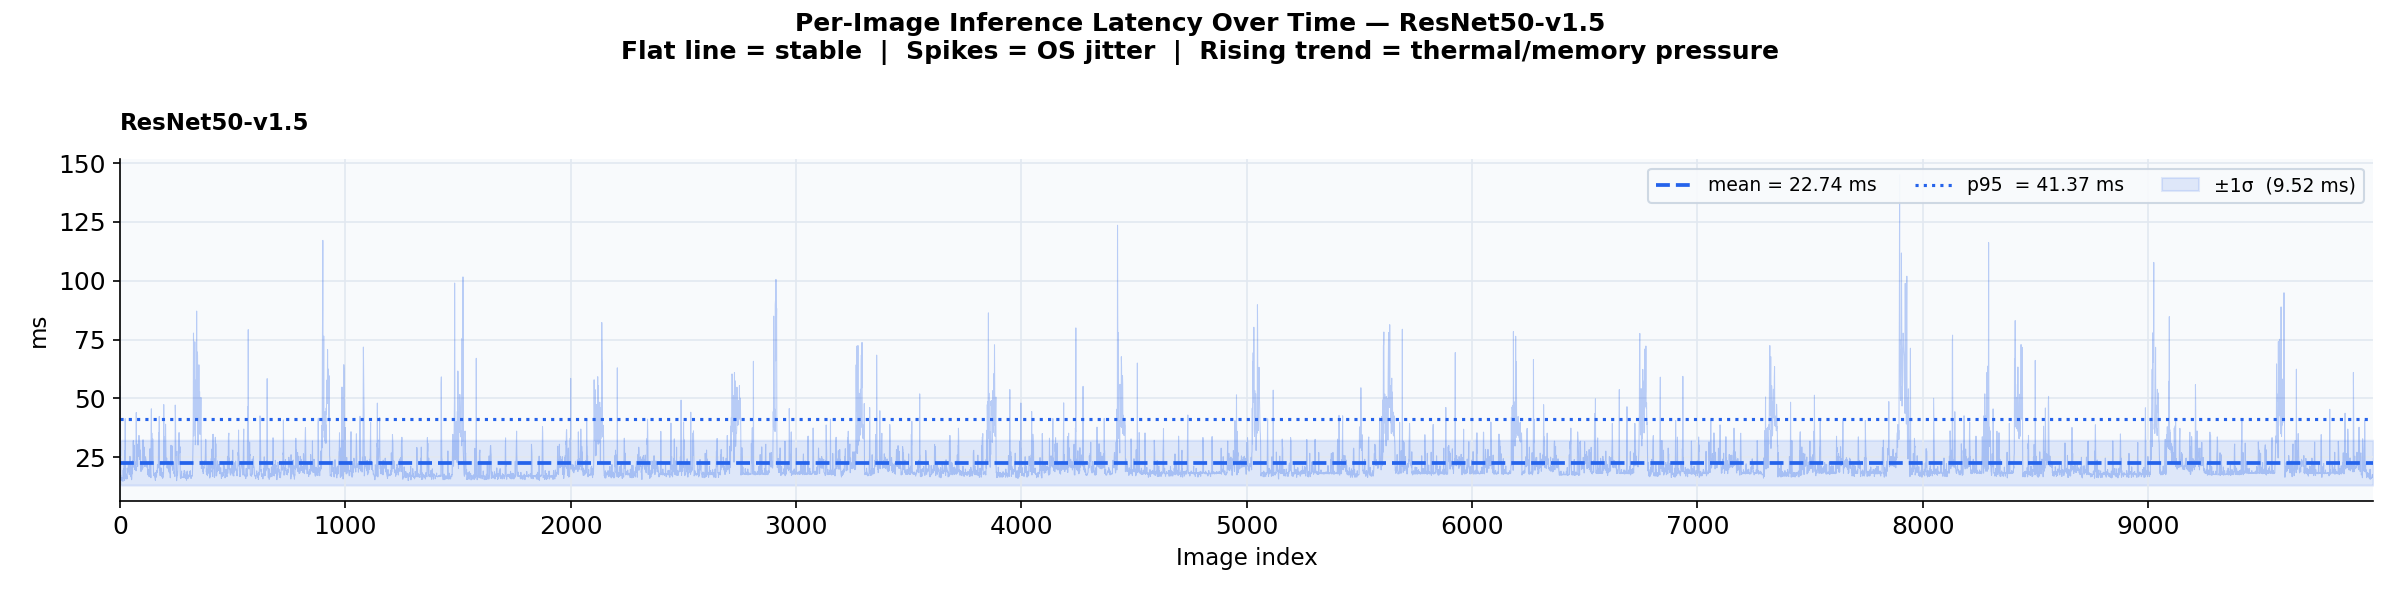
\includegraphics[width=\textwidth]{img/pics updated hiararchy pfe/Per-Model Latency Over Time/1-241-1.png}
    \caption{Latency distribution --- ResNet50-v1.5.}
    \label{fig:m1_hist_resnet50}
\end{figure}

\begin{figure}[p]
    \centering
    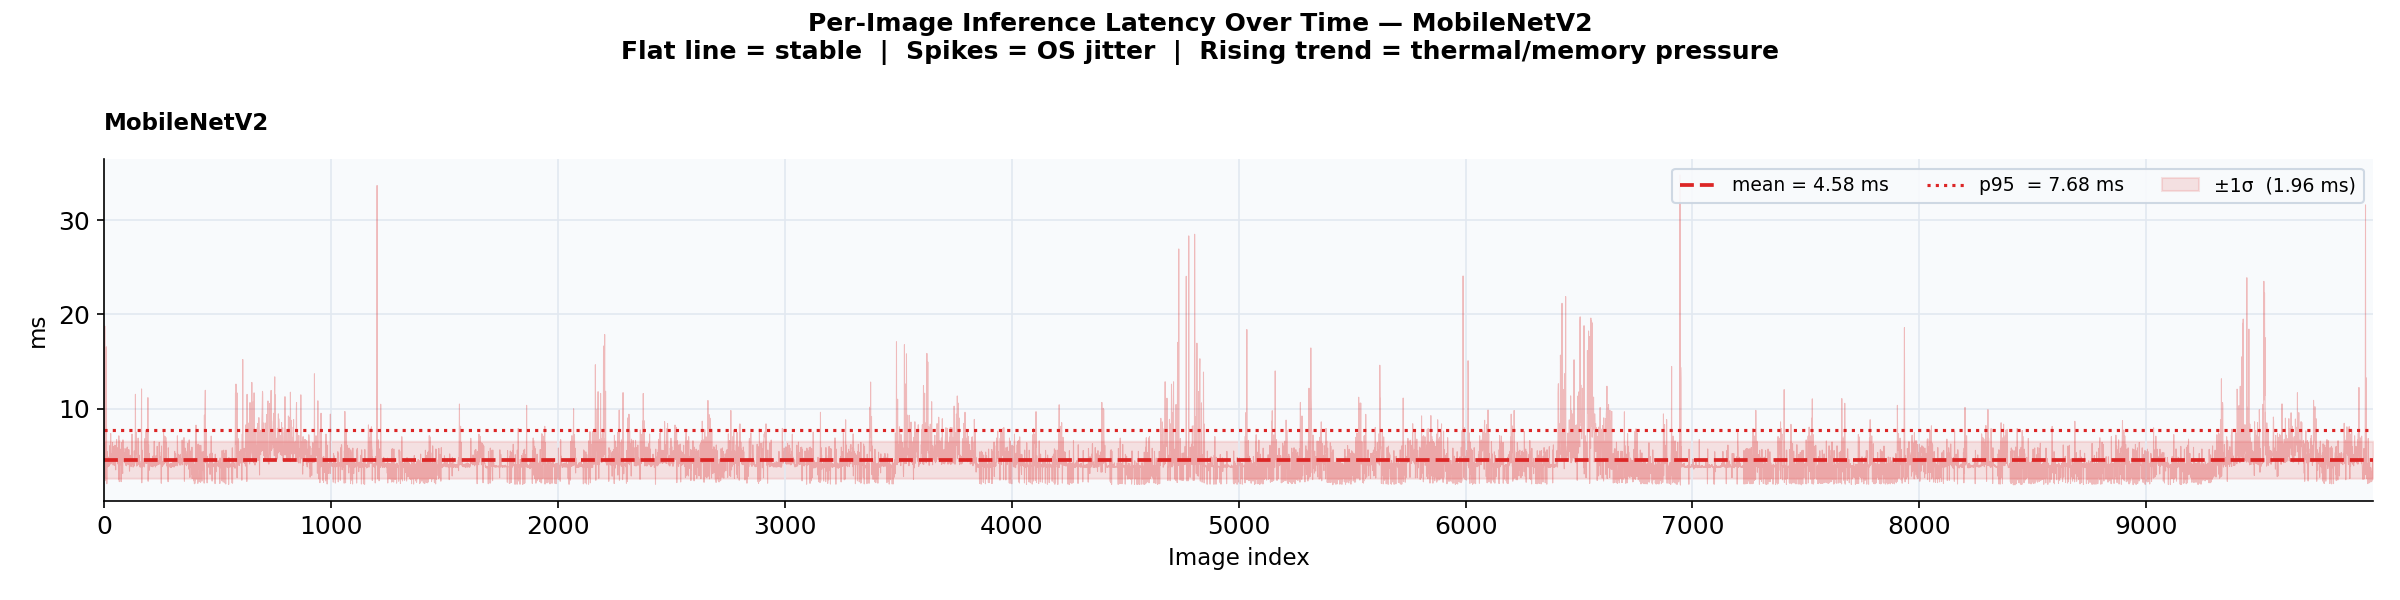
\includegraphics[width=\textwidth]{img/pics updated hiararchy pfe/Per-Model Latency Over Time/1-241-2.png}
    \caption{Latency distribution --- MobileNetV2.}
    \label{fig:m1_hist_mbv2}
\end{figure}

\begin{figure}[p]
    \centering
    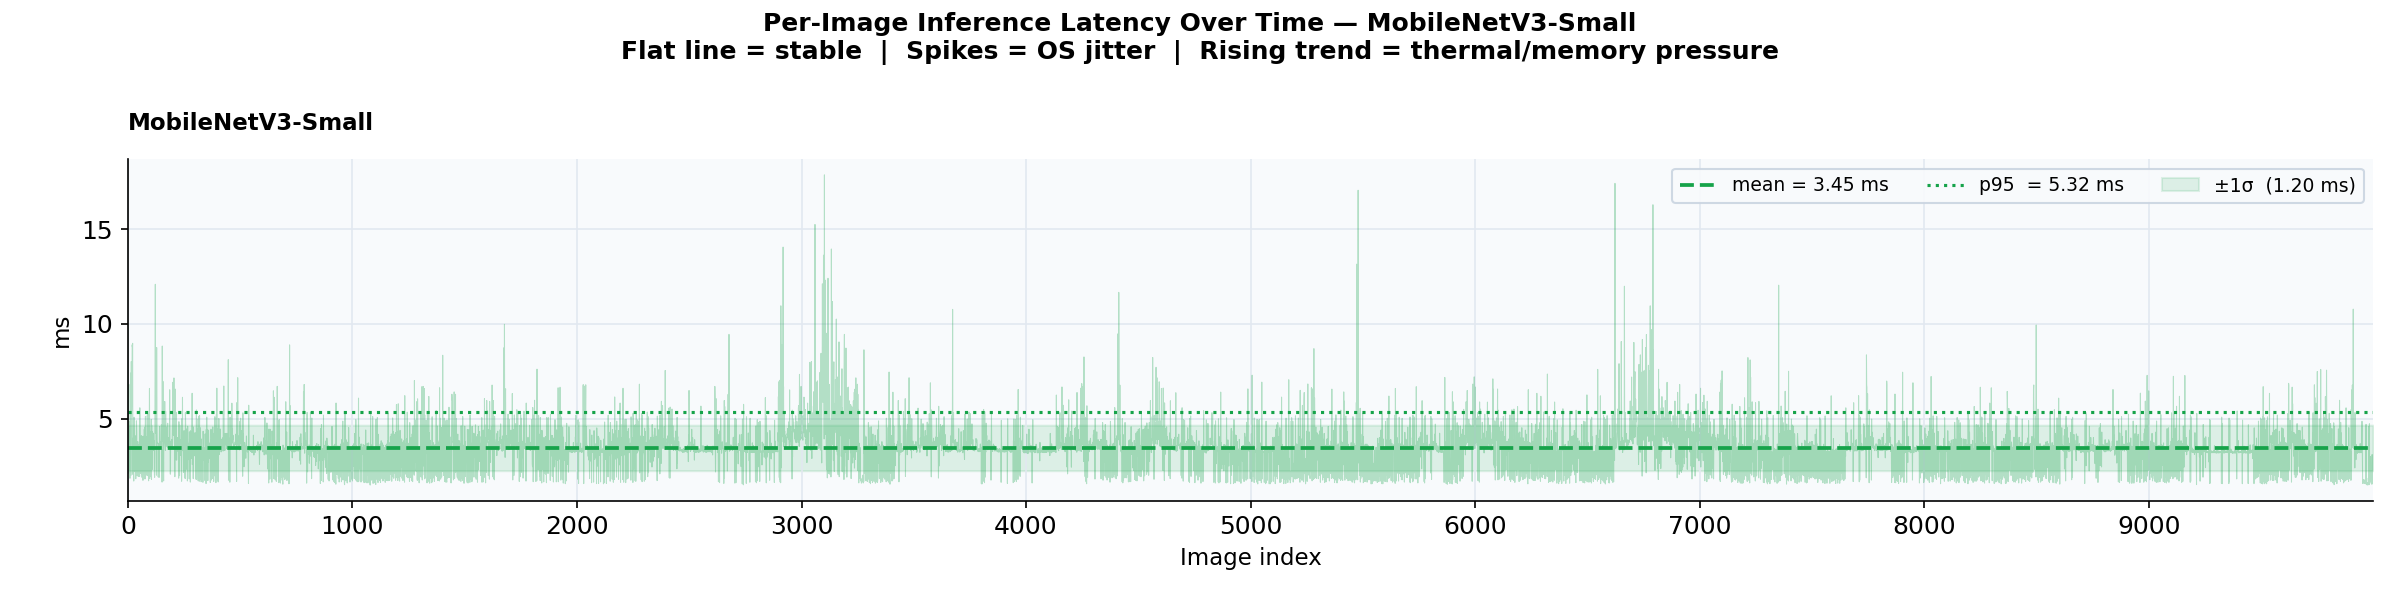
\includegraphics[width=\textwidth]{img/pics updated hiararchy pfe/Per-Model Latency Over Time/1-241-3.png}
    \caption{Latency distribution --- MobileNetV3-Small.}
    \label{fig:m1_hist_mbv3small}
\end{figure}

\begin{figure}[p]
    \centering
    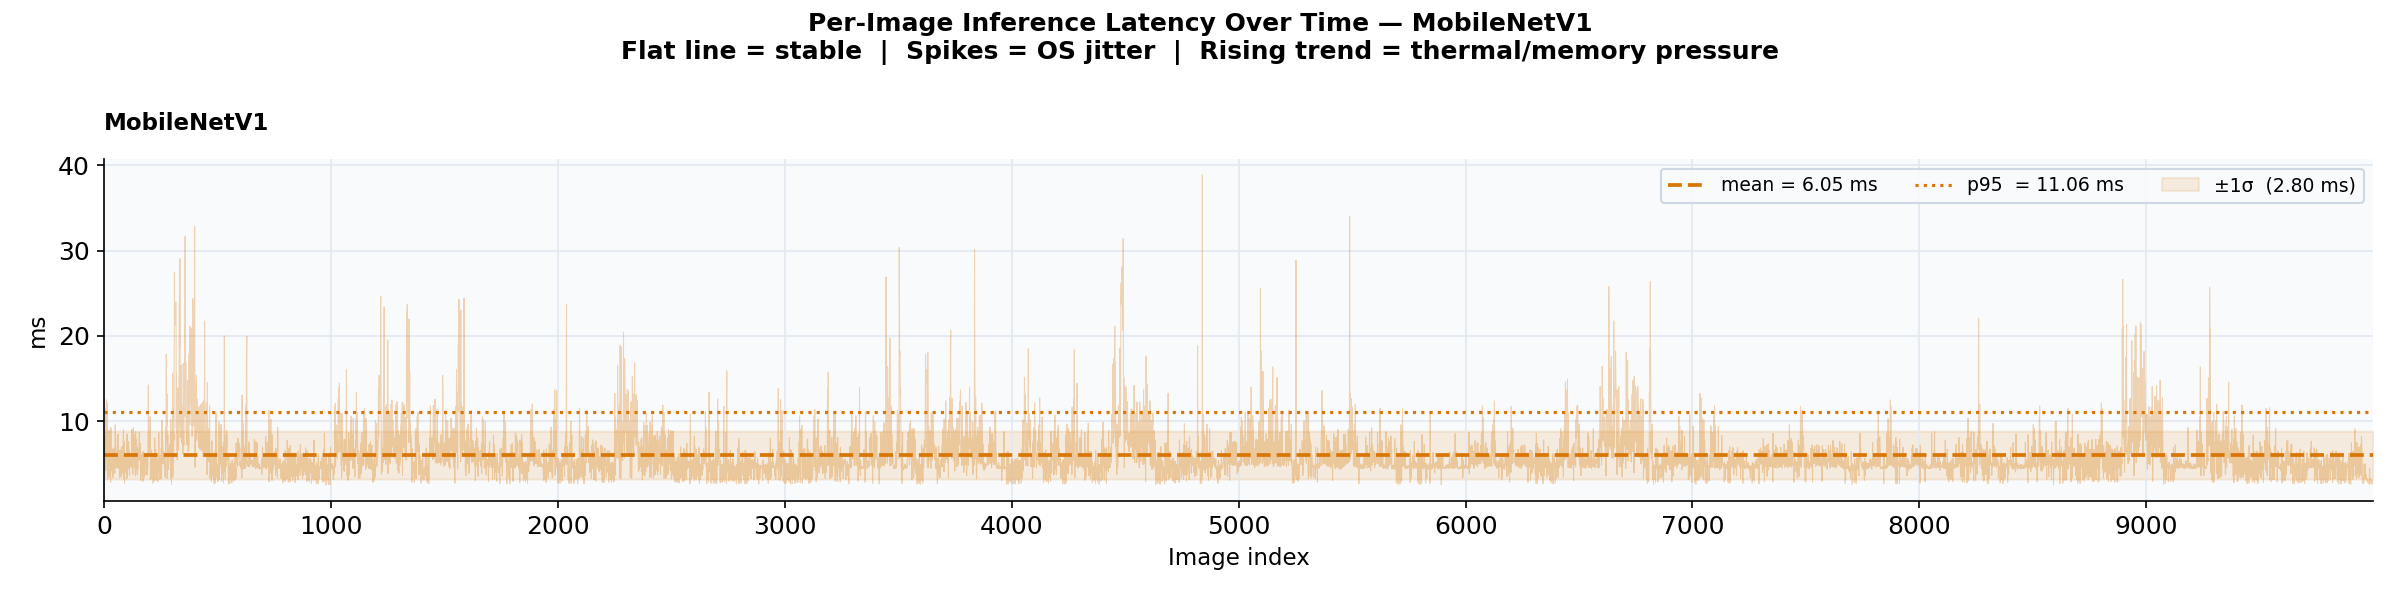
\includegraphics[width=\textwidth]{img/pics updated hiararchy pfe/Per-Model Latency Over Time/1-241-4.png}
    \caption{Latency distribution --- MobileNetV1.}
    \label{fig:m1_hist_mbv1}
\end{figure}

\begin{figure}[p]
    \centering
    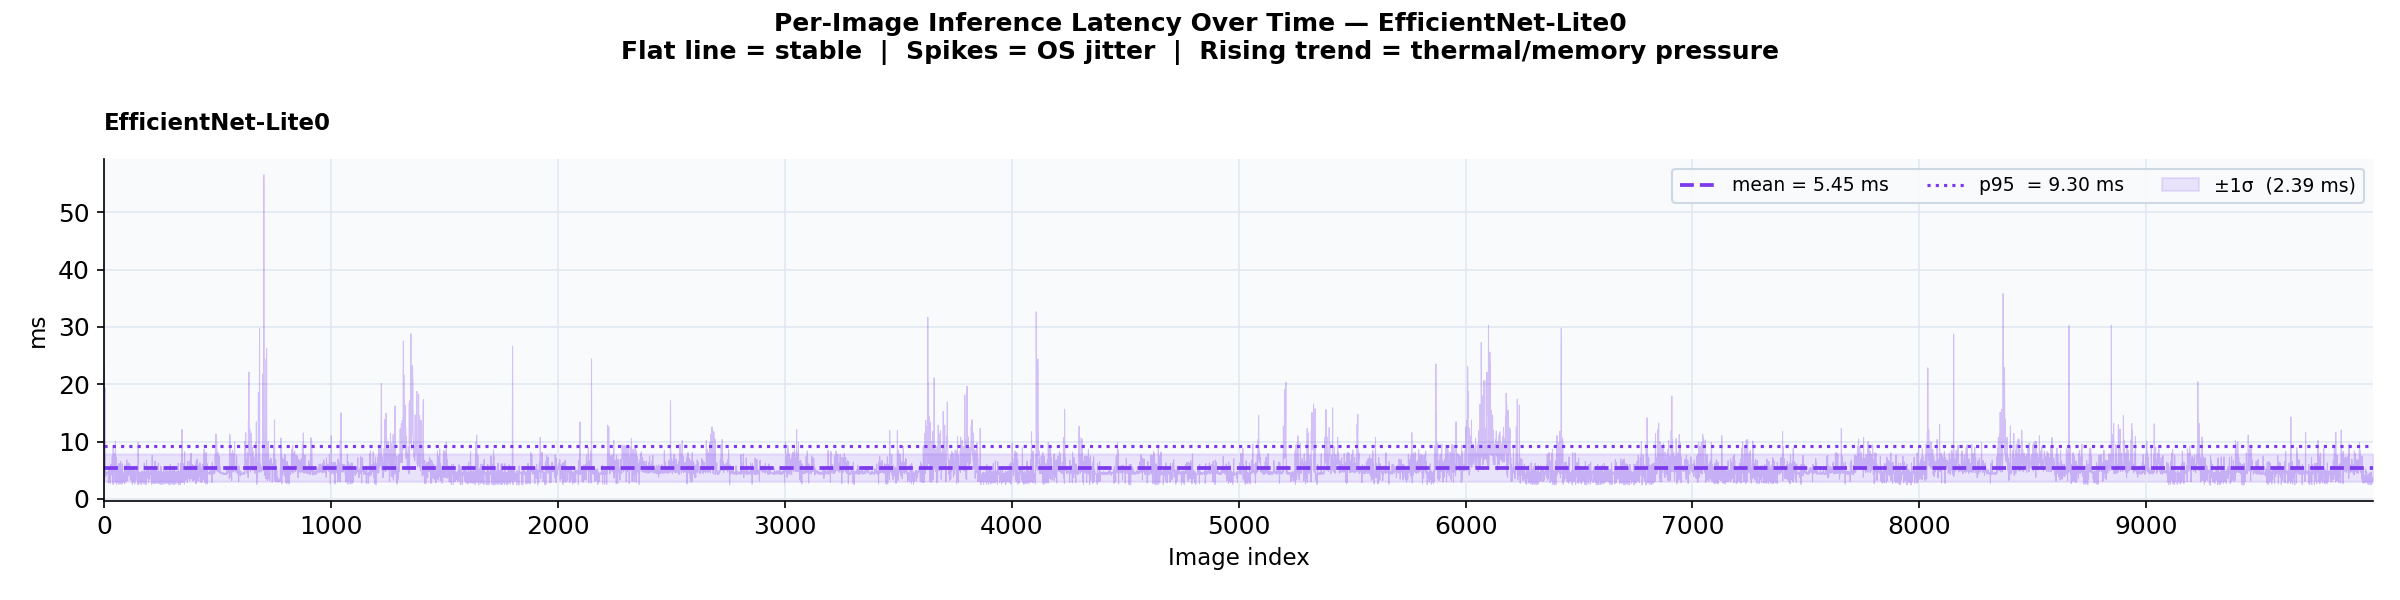
\includegraphics[width=\textwidth]{img/pics updated hiararchy pfe/Per-Model Latency Over Time/1-241-5.png}
    \caption{Latency distribution --- EfficientNet-Lite0.}
    \label{fig:m1_hist_effnet}
\end{figure}

\begin{figure}[p]
    \centering
    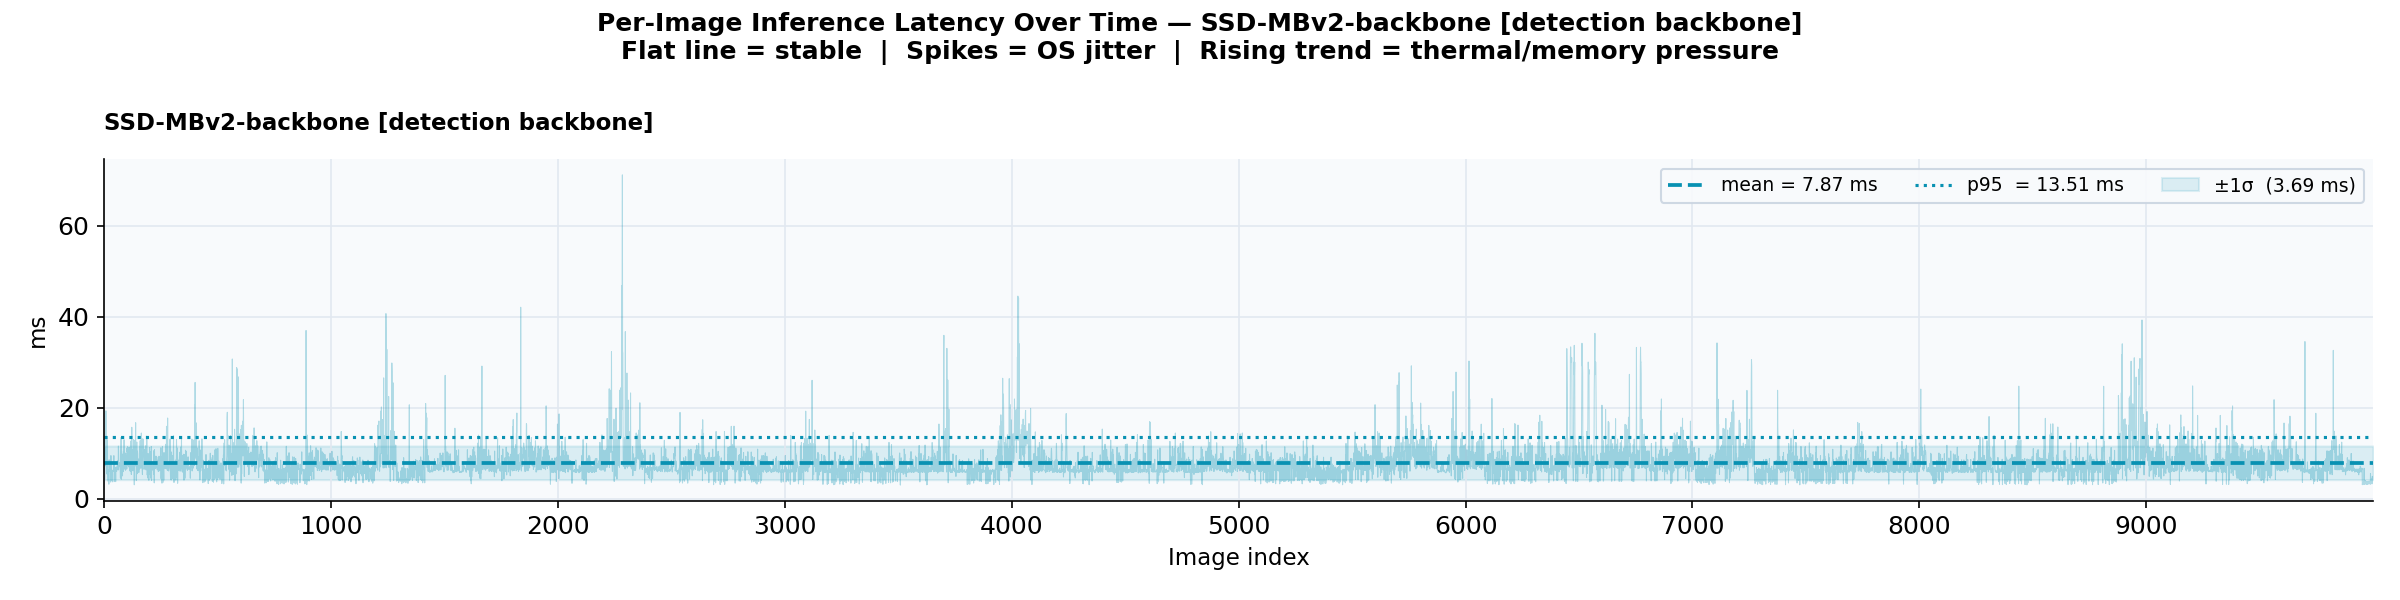
\includegraphics[width=\textwidth]{img/pics updated hiararchy pfe/Per-Model Latency Over Time/1-241-6.png}
    \caption{Latency distribution --- SSD-MBv2-backbone.}
    \label{fig:m1_hist_ssd}
\end{figure}

\clearpage  % flush all remaining floats before continuing

\subsection{Validity Scope and Limitations}

\subsection{Validity Scope and Limitations}

\begin{description}[itemsep=1pt, topsep=3pt]
    \item[\textbf{CPU simulator validity.}] Absolute error versus real
          hardware is expected to be within $\pm15\%$ for mean latency,
          pending physical validation.
    \item[\textbf{NPU simulator validity.}] NPU latency estimates are
          indicative only. They assume perfect INT8 calibration and full
          operator support. Unsupported operators would fall back to CPU,
          increasing real latency.
    \item[\textbf{Accuracy.}] All accuracy numbers derive from real
          \texttt{float32} forward passes. INT8 quantisation effects on
          accuracy must be evaluated on physical hardware with the NXP eIQ
          toolkit.
\end{description}

% =============================================================================
\section{Methodology 3: QEMU User-Mode ARM64 Emulation}
\label{sec:m3_design}
% =============================================================================

\subsection{Overview and Motivation}

Methodology~3 attempts to \emph{actually execute} real ARM64 machine code on
the x86 host using QEMU's user-mode emulation
(\texttt{qemu-aarch64-static}), inside a Docker container running a genuine
ARM64 build of ONNX Runtime. As documented below, QEMU's translation overhead
completely dominates the measured execution time, making this approach
infeasible for inference benchmarking.

\subsection{Two-Stage Docker Image Build}

\begin{enumerate}[itemsep=1pt, topsep=3pt]
    \item \textbf{Stage~A — ARM64 builder:} A genuine \texttt{linux/arm64}
          Ubuntu~22.04 image produces authentic AArch64 ELF binaries:
          Python~3.10, \texttt{numpy}~1.24.4, \texttt{Pillow}~10.4.0, and
          \texttt{onnxruntime}~1.16.3.
    \item \textbf{Stage~B — x86 runner:} Starting from \texttt{amd64}
          Ubuntu~22.04, the ARM64 files are copied into
          \texttt{/opt/arm64\_sysroot/}. The \texttt{qemu-aarch64-static}
          binary is registered with the kernel via \texttt{binfmt\_misc} for
          transparent ARM64 interception.
\end{enumerate}

A wrapper script \texttt{arm64-python} launches the ARM64 Python interpreter
through QEMU with \texttt{OMP\_NUM\_THREADS=4} and
\texttt{ORT\_NUM\_THREADS=4}, mirroring the four-core Cortex-A53 cluster.

\begin{lstlisting}[language=bash,
    caption={The \texttt{arm64-python} wrapper script.}]
#!/bin/bash
exec qemu-aarch64-static \
    -L /opt/arm64_sysroot \
    -E "LD_LIBRARY_PATH=/opt/arm64_sysroot/usr/lib/aarch64-linux-gnu:..." \
    -E OMP_NUM_THREADS=4 \
    -E ORT_NUM_THREADS=4 \
    /opt/arm64_sysroot/usr/bin/python3.10 "$@"
\end{lstlisting}

\subsection{Pipeline Stages}

The orchestrator (\texttt{lrun\_benchmark.py}) runs six stages:
Stage~1 (Docker build), Stage~2 (setup: data download, ONNX export, config),
Stage~2b (ARM64 execution verification via \texttt{platform.machine()}),
Stage~3 (ARM64 inference via \texttt{linference\_qemu\_native.py}),
Stage~4 (statistical metrics), and Stage~5 (visualisation).

\subsection{Observed Failure and Root-Cause Analysis}

Stages~1 and~2 completed normally. Stage~3 correctly printed
\texttt{machine=aarch64} and loaded the ONNX model in $\approx18{,}340$~ms.
The three-run warm-up loop then started and did not return within one hour, at
which point the pipeline was manually terminated.

Three compounding factors explain the extreme slowdown:

\begin{enumerate}[itemsep=1pt, topsep=3pt]
    \item \textbf{Translation overhead:} Every ARM64 instruction block not
          previously seen must be decoded and translated to x86 before
          execution. A single ResNet-50 forward pass involves tens of millions
          of unique instruction sequences on the first call.
    \item \textbf{NEON SIMD emulation:} ONNX Runtime's ARM MLAS kernels use
          ARM NEON (128-bit SIMD) intrinsics. QEMU TCG decomposes each
          128-bit NEON instruction into many scalar x86 operations.
    \item \textbf{No host AVX acceleration:} The ARM64 MLAS kernels are
          compiled for AArch64 only. Even though the host CPU has AVX2, QEMU
          cannot redirect the ARM code to use it.
\end{enumerate}

\begin{table}[H]
\centering
\caption{Summary of Methodology~3 outcomes.}
\label{tab:m3_summary}
\begin{tabular}{ll}
\toprule
\textbf{Attribute} & \textbf{Value / Outcome} \\
\midrule
Emulation mode            & QEMU TCG user-mode (\texttt{qemu-aarch64-static}) \\
Host architecture         & x86\_64 Linux \\
Guest architecture        & AArch64 (ARMv8-A) \\
ORT version               & 1.16.3 (AArch64 native binary) \\
Warm-up runs configured   & 3 \\
Warm-up completion status & Not completed within 1~hour \\
Decision                  & \textbf{Aborted --- approach not viable} \\
\bottomrule
\end{tabular}
\end{table}

\subsection{Lessons Learned}

QEMU TCG is excellent for functional testing and software porting but provides
no timing fidelity relative to real ARM64 silicon. For workloads dominated by
large matrix multiplications inside ONNX Runtime's ARM NEON MLAS kernels, the
gap between QEMU TCG speed and real hardware speed is so large that measured
latencies carry no practical meaning for embedded deployment decisions. The
physics-based simulation of Methodology~2 produces grounded latency estimates
in minutes rather than hours.

% =============================================================================
\section{Architectural Design}
\label{sec:architectural_design}
% =============================================================================

\subsection{Physical Architecture}

The benchmarking environment spans a host x86-64 workstation running the
physics-based simulators (Methodology~2), the ONNX Runtime x86 installation
(Methodology~1), and the Docker engine providing the containerised ARM64
environment (Methodology~3).

% ---- PLACEHOLDER: Physical architecture diagram ----
% A block diagram showing: Host PC -> [M1: ORT x86 | M2: ARMCPUSimulator +
% ARMNPUSimulator | M3: Docker + QEMU] -> Simulated i.MX8M Plus
% \begin{figure}[H]
%     \centering
%     \includegraphics[width=\textwidth]{vis/physical_architecture.png}
%     \caption{Physical architecture of the emulation and simulation
%              environment.}
%     \label{fig:physical_arch}
% \end{figure}

\subsection{Data Flow Architecture}

\begin{enumerate}[itemsep=1pt, topsep=3pt]
    \item ONNX models and Tiny-ImageNet dataset are prepared once and shared
          across all methodologies.
    \item Each methodology executes inference and writes raw latency vectors
          to JSON files.
    \item Metrics scripts compute statistical summaries and write CSV files.
    \item Visualisation scripts generate comparative plots from JSON/CSV.
\end{enumerate}

% =============================================================================
\section{Technology Choices}
\label{sec:technology_choices}
% =============================================================================

\subsection{Why ONNX Runtime}

ONNX Runtime provides cross-platform execution providers
(\texttt{CPUExecutionProvider} for x86 and ARM CPU,
\texttt{VsiNpuExecutionProvider} for Vivante NPU) through a unified API,
enabling direct comparison across hardware targets using the same model files.
Opset~17 covers all selected architectures. ONNX Runtime is the reference
engine for MLPerf~Tiny, ensuring methodology alignment with industry-standard
benchmarks.

\subsection{Why Physics-Based Simulation over Pure QEMU Emulation}

The failure of Methodology~3 empirically validated the physics-based approach:
(1) \textbf{computational feasibility} — full 10\,000-image benchmark in
minutes versus infeasible multi-day QEMU runtime; (2) \textbf{timing fidelity}
— latency estimates grounded in real micro-architectural parameters rather than
emulator overhead; (3) \textbf{configurability} — all parameters exposed in a
single JSON file; (4) \textbf{transparency} — each physical effect is a
separate, documented step.

\subsection{Why the Two-Pass Calibration Strategy}

The 200-image calibration pass resolves the circular dependency between the
ARM CPU and NPU simulators at minimal cost (2\% of the full dataset), providing
a stable estimate of $\bar{L}_{\text{ARM}}^{\text{calib}}$.

\subsection{Simulation Parameter Choices}

Key parameter justifications:
\begin{itemize}[itemsep=1pt, topsep=3pt]
    \item $p_{\text{mem}}=4\%$: midpoint of the 3--5\% contention rate
          reported for i.MX~8 family boards under typical Yocto Linux load.
    \item $f_{\text{mem}}=1.35$: upper end of the 30--40\% stall penalty
          reported in NXP i.MX~8M~Plus application notes.
    \item $\text{CV}_{\text{NPU}}=3\%$: consistent with NXP eIQ benchmark
          reports on the GC7000UltraLite (2--4\% range).
    \item $p_w=15\%$: based on LPDDR4/L2 latency ratio
          ($\sim60$~ns\,/\,$\sim10$~ns) and proportion of memory-bound
          operations in MobileNet-family models.
    \item Thermal onset at image~200: reflects the $\sim30$--60~s
          steady-state warm-up time of embedded SoCs at typical frame rates.
\end{itemize}

% =============================================================================
\section{Comparative Results}
\label{sec:m_results}
% =============================================================================

\subsection{Methodology Comparison}

\begin{table}[H]
\centering
\caption{Summary comparison of the three benchmarking methodologies.}
\label{tab:method_compare}
\resizebox{\textwidth}{!}{%
\begin{tabular}{lccc}
\toprule
\textbf{Attribute} & \textbf{Methodology~1} & \textbf{Methodology~2}
    & \textbf{Methodology~3} \\
\midrule
Execution target  & x86 CPU (real)    & x86 + ARM sim        & AArch64 (QEMU) \\
Latency type      & Measured          & Measured + simulated & Emulated (aborted) \\
ARM accuracy      & N/A               & $\pm15\%$ (estimated)& Would be exact \\
NPU estimate      & None              & Indicative (INT8)    & None \\
Hardware required & x86 workstation   & x86 workstation      & x86 + Docker \\
Completion status & \textbf{Complete} & \textbf{Complete}    & \textbf{Aborted} \\
Runtime           & $\sim$minutes     & $\sim$minutes        & $\sim$hours--days \\
Primary limitation& No ARM estimate   & Analytic model only  & TCG slowdown \\
\bottomrule
\end{tabular}}
\end{table}

\subsection{Key Findings}

\begin{enumerate}[itemsep=1pt, topsep=3pt]
    \item \textbf{MobileNetV1} and \textbf{EfficientNet-Lite0} are the most
          NPU-compatible architectures ($8.33\times$ and $7.14\times$ speedup,
          respectively).
    \item \textbf{MobileNetV3-Small} achieves the lowest x86 latency
          (3.45~ms) but its SE blocks reduce NPU efficiency ($5.00\times$
          speedup vs.\ $8.33\times$ for V1).
    \item \textbf{ResNet50-v1.5} provides the highest accuracy (30.6\%) but
          is the least efficient on both CPU and NPU due to large weight
          tensors exceeding SRAM capacity.
    \item \textbf{Physics-based simulation} produces actionable latency
          estimates in minutes; QEMU instruction-level emulation is
          computationally infeasible for this workload class.
\end{enumerate}

\subsection{Reproducibility}

The pipeline is fully deterministic given \texttt{seed=42} and the canonical
\texttt{pairing\_manifest.csv} ordering. Results are sensitive to CPU
frequency governor, background workload, ONNX Runtime version, and
Pillow/libjpeg version.

% =============================================================================
\section*{Conclusion}
% =============================================================================

This chapter presented a three-methodology emulation and simulation framework
for benchmarking ONNX model inference targeting the NXP i.MX~8M~Plus.
Methodology~1 established that MobileNetV3-Small offers the best x86 latency
(3.45~ms) while the high CV (0.35--0.47) motivated the embedded deployment
study. Methodology~2 delivered a six-effect physics-based simulation producing
ARM CPU and NPU latency estimates in minutes, identifying MobileNetV1
($8.33\times$ NPU speedup) and EfficientNet-Lite0 ($7.14\times$, 31.7\%
accuracy) as the most NPU-compatible architectures. Methodology~3 was
formally attempted and abandoned after the QEMU TCG warm-up phase exceeded
one hour, providing a concrete data point on the infeasibility of
instruction-level emulation for neural network benchmarking.

The next chapter will present the transition to physical hardware validation,
where the simulation estimates from Methodology~2 will be compared against
real measurements on the NXP i.MX~8M~Plus board.
        \clearpage
        
        \input{chap_04}
        \clearpage
        
        \input{conclusion}
        \clearpage
        
        % @author: Stoufa
		% the command `\nocite{*}` is mandatory to avoid the “no \citation commands” error
        % https://tex.stackexchange.com/questions/18045/problem-with-compiling-bibtex-no-citation-commands-error
        %\nocite{*}
        \printbibliography[heading=bibintoc]
        
        \input{annexes}
        \clearpage

    \backmatter
        \input{./tpl/resume}
    
\end{document}